 
% SOSTITUIRE "PATH" CON IL PERCORSO CHE PERMETTE DI ARRIVARE ALLA CARTELLA "Latex"

\documentclass[a4paper]{article}

% info gruppo  
\newcommand{\Gruppo}{\textit{Roundabout}}
\newcommand{\Mail}{team.roundabout.13@gmail.com}

% info progetto
\newcommand{\NomeProgetto}{\textit{Etherless}}
\newcommand{\TV}{Prof. Tullio Vardanega}
\newcommand{\RC}{Prof. Riccardo Cardin}
\newcommand{\Proponente}{\textit{RedBabel}}


% membri del gruppo 
\newcommand{\VB}{Veronica Barbieri}
\newcommand{\LB}{Luca Benetazzo}
\newcommand{\NF}{Nicoletta Fabro}
\newcommand{\EG}{Egon Galvani}
\newcommand{\FJ}{Feim Jakupi}
\newcommand{\MP}{Marco Positello}
\newcommand{\AS}{Alessandro Sgreva}
\newcommand{\AZ}{Antonio Zlatkovski}

% documenti
\newcommand{\SdF}{\textit{Studio di Fattibilità}}
\newcommand{\PdQ}{\textit{Piano di Qualifica}}
\newcommand{\PdP}{\textit{Piano di Progetto}}
\newcommand{\NdP}{\textit{Norme di Progetto}}
\newcommand{\AdR}{\textit{Analisi dei Requisiti}}
\newcommand{\Glossario}{\textit{Glossario}}
\newcommand{\TB}{\textit{Technology Baseline}}
\newcommand{\PB}{\textit{Product Baseline}}
\newcommand{\Verbale}{\textit{Verbale}}

%Lista dei comandi personalizzati
\newcommand{\docTitle}{Analisi dei requisiti}
\newcommand{\docVersion}{1.0.3}
\newcommand{\approv}{}
\newcommand{\ver}{\FJ{} \\ & \MP{} \\ & \AZ{}\\ & \NF{}}
\newcommand{\red}{\EG{} \\ & \AZ{}}
\newcommand{\state}{Non approvato}
\newcommand{\use}{Esterno}
\newcommand{\desc}{Analisi dei requisiti del gruppo \Gruppo{} per la realizzazione del progetto \NomeProgetto}
\newcommand{\destinatari}{\Gruppo\\&\Proponente\\& Prof. Tullio Vardanega\\& Prof. Riccardo Cardin}

\newcommand{\ug}{utente generico}
\newcommand{\ua}{utente autenticato}
\newcommand{\una}{utente non autenticato}
\newcommand{\us}{utente sviluppatore}
\newcommand{\re}{rete Ethereum\ped{\textit{G}}}

\newcommand{\help}{\texttt{help}}
\newcommand{\init}{\texttt{init}}
\newcommand{\login}{\texttt{login}}
\newcommand{\signup}{\texttt{signup}}
\newcommand{\logout}{\texttt{logout}}
\newcommand{\whoami}{\texttt{whoami}}
\newcommand{\lista}{\texttt{list}}
\newcommand{\deploy}{\texttt{deploy}}
\newcommand{\run}{\texttt{run}}
\newcommand{\info}{\texttt{info}}
\newcommand{\search}{\texttt{search}}
\newcommand{\delete}{\texttt{delete}}
\newcommand{\history}{\texttt{history}}
\newcommand{\edit}{\texttt{edit}}

\newcommand{\phelp}{\texttt{command\_name -{}-help}}
\newcommand{\ploginPrivate}{ \texttt{login private\_key password} }
\newcommand{\ploginMnemonic}{\texttt{login mnemonic\_phrase password}}
\newcommand{\pdeploy}{\texttt{deploy file\_path function\_name desc}}
\newcommand{\prun}{\texttt{run function\_name [parameters\_list]}}
\newcommand{\pinfo}{\texttt{info function\_name}}
\newcommand{\psearch}{\texttt{search keyword}}
\newcommand{\pdelete}{\texttt{delete function\_name}}
\newcommand{\plista}{\texttt{list -m}}
\newcommand{\pedit}{\texttt{edit function\_name}}

\newcommand{\ucs}{0.19}

% comandi per i requisiti
\newcommand{\ob}{Obbligatorio}
\newcommand{\de}{Desiderabile}
\newcommand{\op}{Opzionale}

% pacakges 
\usepackage{geometry}
\usepackage{hyperref} %  link
\usepackage{graphicx} %immagini
\usepackage{titlesec} %per creazione di una section personalizzata
\usepackage{float} %per il posizionamento delle figure

% package per la lingua / caratteri 
\usepackage[italian]{babel} 
\usepackage[utf8]{inputenc}
\usepackage[T1]{fontenc}

\usepackage{fancyhdr} % per header e footer 
\usepackage{lastpage} % per avere l'indice dell'ultima pagina 

\usepackage{tabularx} % tabelle
\usepackage[table]{xcolor} % definizione colore di sfondo per tabelle
\usepackage{longtable} % permette di estendere le tabelle su più pagine  

\usepackage{chngcntr} % per numerazione immagini e tabelle 

% configurazione
% link
\hypersetup{
	colorlinks=true,
	linkcolor=black,
	filecolor=magenta,      
	urlcolor=blue,
}

% intestazione e piè di pagina 
\pagestyle{fancy}
% intestazione 
\setlength{\headheight}{25pt}
\lhead{ 
\includegraphics[scale=0.05]{./res/img/cropped_logo.png} } 
\rhead{ \docTitle } 
% piè di pagina \\
\renewcommand{\footrulewidth}{0.4pt} % per avere una linea nel footer
\cfoot{}
\rfoot{Pagina \thepage{} di \pageref{LastPage}}

% tabelle 
\def\arraystretch{1.5} % padding 
% comandi e colori tabelle
\definecolor{lightRowColor}{HTML}{fafafa}
\definecolor{darkRowColor}{HTML}{ffcccb}

\newcommand{\coloredTableHead}{\rowcolor[HTML]{b61827}}
\newcommand{\lightTableRow}{\rowcolor{lightRowColor}}
\newcommand{\darkTableRow}{\rowcolor{darkRowColor}}

% per numerazione immagini e tabelle 
% --> la numerazione dipende dalla subsection in cui ci si trova 
\counterwithin{table}{subsection}
\counterwithin{figure}{subsection}

% definizione del comando subsubsubsection
\titleclass{\subsubsubsection}{straight}[\subsection]

\newcounter{subsubsubsection}[subsubsection]
\renewcommand\thesubsubsubsection{\thesubsubsection.\arabic{subsubsubsection}}

\titleformat{\subsubsubsection}
  {\normalfont\normalsize\bfseries}{\thesubsubsubsection}{1em}{}
\titlespacing*{\subsubsubsection}
{0pt}{3.25ex plus 1ex minus .2ex}{1.5ex plus .2ex}

\makeatletter
\def\toclevel@subsubsubsection{4}
\def\toclevel@paragraph{5}
\def\toclevel@paragraph{6}
\def\l@subsubsubsection{\@dottedtocline{4}{7em}{4em}}
\def\l@paragraph{\@dottedtocline{5}{10em}{5em}}
\def\l@subparagraph{\@dottedtocline{6}{14em}{6em}}
\makeatother

\setcounter{secnumdepth}{4}
\setcounter{tocdepth}{4}

\usepackage{array}
\newcolumntype{C}{>{\centering\arraybackslash}p{11.28cm}}

\begin{document}

	% copertina 
	\thispagestyle{empty}
\begin{titlepage}
	\begin{center}
		
\includegraphics[scale=0.25]{./res/img/logo.png}\\
		\large \textbf{\Gruppo\hspace{1.5mm}-\hspace{1.5mm}\NomeProgetto}
		\vfill
		\Huge \textbf{\docTitle}
		\vspace*{\fill}
        \vfill
        \large

        \begin{tabular}{r|l}
			\textbf{Versione} & \docVersion \\
			\textbf{Approvazione} & \approv \\
			\textbf{Redazione} & \red \\
			\textbf{Verifica} & \ver \\
			\textbf{Stato} & \state \\
			\textbf{Uso} & \use \\
			\textbf{Destinato a} & \destinatari\\
		\end{tabular}

		\vfill
		\normalsize
		\textbf{Descrizione}\\
		\textit{\desc} \\
		\vfill
		\small\texttt{\Mail}
	\end{center}
\end{titlepage}

	
	% diario delle modifiche 
	\section*{Changelog} % con section* evito che la sezione sia considerata nell'indice

\rowcolors{2}{lightRowColor}{darkRowColor}
\begin{longtable}{
		>{\centering}p{0.05\textwidth}	%Versione
		>{\centering}p{0.13\textwidth}	%Data
		>{\centering}p{0.22\textwidth}	%Nominativo
		>{}p{0.24\textwidth}			%Descrizione
		>{\centering}p{0.22\textwidth} }	%Verifica

	\coloredTableHead
	\textbf{\color{white}V} &
	\textbf{\color{white}Date} &
	\textbf{\color{white}Name} &
	\textbf{\color{white}Description} &
	\textbf{\color{white}Check}
	\tabularnewline
	\endhead

	% contenuto tabella
	% Versione & data & Nome \\ Ruolo & Descrizione & Verificatore \\ Ruolo
	1.0.0 & 2020-07-16 & \NF \\ \textit{Project manager} & Approved the document with no retrocompatible changes.& \tabularnewline
	0.2.0 & 2020-07-14 & \AS \\ \textit{Verifier} & Verified the whole document with corrections.& \tabularnewline
	0.1.3 & 2020-07-09 & \MP \\ \textit{Developer} & Updated section \textsection{4} & \NF{} \\ \textit{Verifier} \tabularnewline
	0.1.2 & 2020-07-07 & \NF \\ \textit{Developer} & Modified section \textsection{2.2} & \EG{} \\ \textit{Verifier} \tabularnewline
	0.1.1 & 2020-07-05 & \NF \\ \textit{Developer} & Modified structure of section \textsection{3} and added content & \EG{} \\ \textit{Verifier} \tabularnewline
	0.1.0 & 2020-06-10 & \AZ \\ \textit{Verifier} & Verified the whole document.& \tabularnewline
	0.0.3 & 2020-06-08 & \VB \\ \textit{Developer} & Added section \textsection{2} and \textsection{4} & \AZ \\ \textit{Verifier} \tabularnewline
	0.0.2 & 2020-06-07 & \FJ \\ \textit{Developer} & Added the commands description in \textsection{3} & \AZ \\ \textit{Verifier} \tabularnewline
	0.0.1 & 2020-05-21 & \NF \\ \textit{Developer} & Created the structure of the document. & \EG \\ \textit{Verifier} \tabularnewline

\end{longtable}

	\pagebreak
	
	% indice 
	\tableofcontents 
	\pagebreak
	
	% lista delle figure
	\listoffigures
	\pagebreak
	
	% lista delle tabelle 
	\listoftables
	\pagebreak
		
	% sezioni 
	\section{Introduzione}
\subsection{Scopo del documento}
Questo documento viene redatto con lo scopo di presentare la pianificazione del gruppo \Gruppo{} per lo sviluppo del progetto \NomeProgetto{}. Vengono inoltre presentate un'analisi dei rischi e un'analisi dei costi riguardanti lo sviluppo del progetto.\\
Nel dettaglio i punti definiti nel documento sono:
\begin{itemize}
	\item analisi dei rischi relativi allo sviluppo del progetto;
	\item breve analisi del modello di sviluppo del progetto;
	\item pianificazione dettagliata dei tempi e delle attività;
	\item stima preventiva dell'utilizzo delle risorse disponibili.
\end{itemize}
\subsection{Scopo del prodotto}
Si svuole sviluppare una piattaforma cloud\ped{\textit{G}} che consenta agli sviluppatori di effettuare il deploy\ped{\textit{G}} di funzioni Javascript\ped{\textit{G}} e gestisca il pagamento per la loro esecuzione tramite la piattaforma Ethereum\ped{\textit{G}}.\\
Il prodotto\ped{\textit{G}} finale prevede quindi l'integrazione di due tecnologie, Serverless\ped{\textit{G}} e Ethereum\ped{\textit{G}}.\\
Il lato Serverless\ped{\textit{G}} si occupa dell'esecuzione delle funzioni fornite dagli sviluppatori. Tali funzioni vengono salvate ed eseguite in un servizio cloud\ped{\textit{G}} esterno, quale Amazon Web Services\ped{\textit{G}}.\\
La richiesta di utilizzo di una funzione e il successivo pagamento vengono invece gestiti tramite la piattaforma Ethereum\ped{\textit{G}} sfruttando gli smart contract\ped{\textit{G}}. Il pagamento viene effettuato in ETH\ped{\textit{G}}.\\
Una percetuale significativa di ogni pagamento viene riservata agli amministratori del servizio.\\
Lo sviluppatore e l'utente finale interagiscono con il prodotto\ped{\textit{G}} tramite una CLI\ped{\textit{G}} che prevede alcuni comandi intuitivi che permettono di usufruire di tutte le funzionalità fornite dalla piattaforma.
\subsection{Glossario}
Al fine di evitare possibili ambiguità, i termini tecnici utilizzati nei documenti formali vengono chiariti ed approfonditi nel \textit{Glossario 4.0.0}. Per facilitare la lettura, i termini presenti in tale documento sono contrassegnati in tutto il resto della documentazione da una 'G' a pedice.
\subsection{Riferimenti}
\subsubsection{Riferimenti normativi}
\begin{itemize}
	\item \textbf{Norme di Progetto}: \textit{Norme di Progetto 4.0.0};
	\item \textbf{Capitolato\ped{\textit{G}} d'appalto Etherless}:\\\url{https://www.math.unipd.it/~tullio/IS-1/2019/Progetto/C2.pdf};
	\item \textbf{Regolamento organigramma di gruppo e specifica tecnico-economica}:\\\url{https://www.math.unipd.it/~tullio/IS-1/2019/Progetto/RO.html}.
\end{itemize}
\subsubsection{Riferimenti informativi}
\begin{itemize}
	\item \textbf{Dispense del corso "Ingegneria del Software" sulla gestione di progetto}:\\\url{https://www.math.unipd.it/~tullio/IS-1/2019/Dispense/L06.pdf};
	\item \textbf{Software Engineering (10th edition) - Ian Sommerville};
	\item \textbf{Guide to the Software Engineering Body of Knowledge (v3) - IEEE Computer Society}.
\end{itemize}
\subsection{Scadenze}
Il gruppo \Gruppo{} ha deciso di rispettare le seguenti scadenze:
\begin{itemize}
	\item \textbf{Revisione dei Requisiti}: 2020-04-13;
	\item \textbf{Revisione di Progettazione}: 2020-05-11;
	\item \textbf{Revisione di Qualifica}: 2020-06-11;
	\item \textbf{Revisione di Accettazione}: 2020-07-13.
\end{itemize}
La pianificazione per lo svolgimento del progetto si basa su queste scadenze.

	\pagebreak
	
	\section{Analisi dei rischi}
\subsection{Gestione dei rischi}
Durante lo sviluppo di un progetto complesso è possibile incorrere in problematiche che potrebbero rallentare o impedire il normale proseguimento del progetto. Risulta quindi necessario effettuare un'approfondita attività di analisi dei fattori di rischio per cercare di evitare o rendere il più ininfluenti possibili le eventuali problematiche che potrebbero presentarsi.
Il risultato di questa analisi è presentata in forma tabellare dove ciascuna voce rappresenta un fattore di rischio ed è costruita tramite le seguenti quattro attività:
\begin{itemize}
		\item \textbf{Individuazione}: vengono identificati i potenziali fattori di rischio che potrebbero causare situazioni problematiche durante lo sviluppo del progetto;
		\item \textbf{Analisi}: viene studiato ciascun fattore di rischio. Questo studio consiste nell'assegnare a ciascun fattore la probabilità che esso si verifichi, un indice di gravità e l'impatto che avrebbe sul progetto nel caso in cui si verifichi;
		\item \textbf{Pianificazione di controllo e mitigazione}: si pianifica una metodologia per evitare che i rischi individuati si verifichino e si stabilisce preventivamente come procedere nel caso in cui il rischio si verifichi. \\
		Questa attività consiste nell'elaborazione di un piano di contingenza per delineare preventivamente le azioni da intraprendere per evitare o mitigare l'insorgere dei problemi individuati;
		\item \textbf{Monitoraggio}: attività continua nella quale la situazione è tenuta sotto controllo per prevenire il verificarsi dei rischi o, nel peggiore dei casi, per intervenire tempestivamente e mitigarli. \\
\end{itemize}


Si è deciso di raggruppare le varie tipologie di fattori di rischio in questo modo:
\begin{itemize}
	\item \textbf{RT}: Rischi Tecnologici;
	\item \textbf{RO}: Rischi Organizzativi;
	\item \textbf{RI}: Rischi Interpersonali;
	\item \textbf{RR}: Rischi legati ai Requisiti.
\end{itemize}

Inoltre per semplificarne la gestione ed evitare possibili ambiguità ciascun rischio verrà identificato da:
\begin{itemize}
	\item ID: [tipologia]-[N] \\
		dove:
		\begin{itemize}
			\item tipologia: una delle tipologie sopra indicate;
			\item N: numero identificativo che, per ciascuna tipologia, parte da 1 e viene incrementato ad ogni nuovo rischio individuato.
		\end{itemize}
	\item nome;
	\item descrizione;
	\item rilevazione;
	\item grado di rischio;
	\item piano di contingenza.
\end{itemize}

\subsection{Rischi preventivati}
\begin{longtable}{
		>{\centering}p{0.15\textwidth}
		>{\centering}p{0.25\textwidth}
		>{\centering}p{0.25\textwidth}
		>{\centering\arraybackslash}p{0.26\textwidth} }

	\rowcolor{white}\caption{Analisi dei  del progetto} \\
	\coloredTableHead
	\textbf{\color{white}ID, Nome e Grado di rischio} &
	\textbf{\color{white}Descrizione} &
	\textbf{\color{white}Rilevazione} &
	\textbf{\color{white}Piano di contingenza}
	\endfirsthead

	\rowcolor{white}\caption[]{(continua)}\\
	\coloredTableHead
	\textbf{\color{white}ID, Nome e Grado di rischio} &
	\textbf{\color{white}Descrizione} &
	\textbf{\color{white}Rilevazione} &
	\textbf{\color{white}Piano di contingenza}
	\endhead

	\hline \multicolumn{4}{c}{\textit{Continua nella prossima pagina}} \\
	\endfoot
	\hline
	\endlastfoot

	% Contenuto tabella
	% Codice & Nome & Descrizione & Rilevamento & Grado di rischio \\

	\rowcolor{lightRowColor}
	RT-1 \\ Tecnologie da utilizzare \\
		\vspace{5mm} %5mm vertical space
	 	Probabilità: \textbf{ALTA} Pericolosità: \textbf{MEDIA}
		&
		Alcune delle tecnologie necessarie allo sviluppo del progetto risultano sconosciute ad alcuni membri del gruppo e inoltre, essendo tecnologie recenti, la documentazione potrebbe essere scarsa o non del tutto completa.
		&
		Ciascun componente del gruppo ha già espresso il livello di conoscenza rispetto a queste teconologie ed è necessario che, non appena qualcuno riscontri un problema riguardo all'uso di qualcuna di esse, lo notifichi immediatamente al resto dei componenti.
		&
		Il Proponente\ped{\textit{G}} e i componenti del gruppo più esperti hanno condiviso del materiale utile per lo studio di queste tecnologie. Nel caso in cui questo materiale si riveli non sufficiente, il Proponente\ped{\textit{G}} si è reso disponibile a chiarire eventuali dubbi che potrebbero insorgere durante lo sviluppo. \\

	\rowcolor{darkRowColor}
	RT-2 \\ Guasti hardware \\
		\vspace{5mm} %5mm vertical space
		Probabilità: \textbf{MEDIA} Pericolosità: \textbf{BASSA}
		&
		Durante lo sviluppo potrebbero esserci malfunzionamenti di uno o più strumenti di lavoro.
		&
		Appena un componente del gruppo nota un malfunzionamento è necessario che lo riferisca agli altri in modo da evitare possibili rallentamenti o impedimenti per il normale proseguimento.
		&
		Se il malfunzionamento non può essere risolto in breve tempo è necessario che il componente del gruppo possa continuare a lavorare su un altro dispositivo. Il cambio di dispositivo è reso molto semplice grazie all'utilizzo di un repository\ped{\textit{G}} GitHub\ped{\textit{G}} e di strumenti collaborativi online. \\
	
	\rowcolor{lightRowColor}
	RT-3 \\ Corretta configurazione dell'ambiente di lavoro \\ 
		Probabilità: \textbf{MEDIA} Pericolosità: \textbf{BASSA}
		&
		Durante lo sviluppo alcuni programmatori potrebbero avere dei problemi nel configurare l'ambiente di sviluppo in modo adeguato. 
		&
		A seguito dell'individuazione di tali difficoltà il programmatore dovrà comunicarle al team tramite gli appositi canali di comunicazione. 
		&
		L'amministratore o altri programmatori che hanno già configurato correttamente l'ambiente di sviluppo in precedenza, dovranno aiutare il programmatore che ha riscontrato tale problema per giungere ad una soluzione in tempi brevi.\\
		
	\rowcolor{darkRowColor}
	RT-4 \\ Conoscenza superficiale dei design pattern e degli stili architetturali \\ 
		Probabilità: \textbf{MEDIA} Pericolosità: \textbf{MEDIA}
		&
		Nel corso della progettazione e  preparazione della Product Baseline è possibile che delle componenti del gruppo non abbiano ancora acquisito le conoscenze necessarie relative a design pattern e stili architetturali. 
		&
		Ogni progettista che si trovi in questa situazione è tenuto a informare il gruppo, e in particolar modo il responsabile. 
		&
		Il responsabile dovrà dialogare con i progettisti, ed eventualmente indicare del materiale adeguato all'apprendimento delle conoscenze necessarie.  \\
	
	\rowcolor{lightRowColor}
	RO-1 \\ Inesperienza \\
		\vspace{5mm} %5mm vertical space
		Probabilità: \textbf{ALTA} Pericolosità: \textbf{MEDIA}
		&
		Tenendo conto della poca esperienza dei componenti del gruppo in un progetto complesso è possibile che non sia semplice per alcuni riuscire ad ambientarsi in questa nuova realtà simile a ciò che succede nel mondo del lavoro.
		&
		È necessario che ciascun componente del gruppo esponga le proprie problematiche così che gli altri componenti possano essere utili per dare un aiuto, in modo da essere il più produttivi possibile.
		&
		È importante che ciscun componente si adoperi per limitare il più possibile eventuali difficoltà o lacune dovute all'inesperienza. \\

	\rowcolor{darkRowColor}
	RO-2 \\ Calcolo dei tempi e dei costi \\
		\vspace{5mm} %5mm vertical space
		Probabilità: \textbf{ALTA} Pericolosità: \textbf{ALTA}
		&
		Rischio causato anche dall'inesperienza sopra esposta. È possibile che i tempi e i costi preventivati si rivelino imprecisi con l'avanzamento del progetto.
		&
		Nel caso in cui un componente riscontri un discostamento dalle ore di lavoro preventivate per ciascuna attività dovrà farlo presente al Responsabile.
		&
		Nel caso in cui una stima oraria risulti non sufficiente per portare a termine una specifica attività, il Responsabile provvederà ad assegnare più risorse in modo da evitare o limitare eventuali rallentamenti al lavoro. Se ciò bastasse e ci dovessero essere variazioni importanti al preventivo iniziale il responsabile provvederà a comunicarlo al Committente\ped{\textit{G}}. \\

	\rowcolor{lightRowColor}
	RO-3 \\ Impegni personali \\
		\vspace{5mm} %5mm vertical space
		Probabilità: \textbf{MEDIA} Pericolosità: \textbf{MEDIA} &
		È presente la possibilità che in alcuni momenti uno o più componenti del gruppo abbiano degli impegni accademici o impegni personali che potrebbero portare ad un rallentamento del lavoro.
		&
		È essenziale che tutti gli impegni vengano notificati al Responsabile appena il componente interessato ne viene a conoscenza.
		&
		Il Responsabile provvederà ad apportare delle modifiche organizzative per evitare o limitare rallentamenti ai lavori. \\
		
	\rowcolor{darkRowColor}
	RO-4 \\ Distribuzione del lavoro disomogenea \\
		\vspace{5mm} %5mm vertical space
		Probabilità: \textbf{BASSA} Pericolosità: \textbf{MEDIA} &
		È possibile che ad uno o più membri del gruppo sia assegnato un compito troppo oneroso, aumentando quindi la probabilità che si verifichino rallentamenti.
		&
		È essenziale che chiunque ritenga di non riuscire a soddisfare entro le scadenze richieste il lavoro assegnato, lo comunichi al resto del gruppo.
		&
		Il Responsabile provvederà a valutare i compiti assegnati ai singoli membri del gruppo e, se necessario, apportare delle modifiche. \\
	
	\rowcolor{lightRowColor}
	RO-5 \\ Approvazione errata dei documenti \\
		\vspace{5mm} %5mm vertical space
		Probabilità: \textbf{BASSA} Pericolosità: \textbf{ALTA} &
		È possibile che il Responsabile durante l'approvazione non si accorga o commetta alcuni errori, portando quindi all'approvazione la consegna di documenti errati. 
		&
		Per ogni documento devono essere eseguiti controlli costanti, in modo che sia possibile identificare in maniera semplice e rapida tali inconsistenze. 
		&
		Il Responsabile si dovrà occupare di controllare che i documenti da approvare siano effettivamente validi. In caso di problemi o errori il responsabile potrà collaborare con un verificatore per risolverli in un tempo adeguato. \\ 
		
	\rowcolor{darkRowColor}
	RO-6 \\ Cattiva gestione dell’archivio per la documentazione del progetto \\
		\vspace{5mm} %5mm vertical space
		Probabilità: \textbf{BASSA} Pericolosità: \textbf{MEDIA} &
		A causa dell'inesperienza dei componenti del gruppo è possibile che alcune funzionalità messe a disposizione dal version control system usato siano poco conosciute. È quindi probabile che si possano verificare problemi ed errori nella gestione della repository. 
		&
		Ogni componente del gruppo che si accorga di tali errori dovrà comunicarli, tramite gli appositi canali di comunicazione, ad un Amministratore. 
		& È richiesto che gli Amministratori abbiano una buona conoscenza dello strumento di versionamento usato, e possano quindi risolvere i problemi individuati in maniera tempestiva. \\
		
	\rowcolor{lightRowColor}
	RI-1 \\ Comunicazioni interne \\
		\vspace{5mm} %5mm vertical space
		Probabilità: \textbf{BASSA} Pericolosità: \textbf{MEDIA} &
		Potrebbero esserci momenti nei quali uno o più componenti potrebbero non essere reperibili. Ciò potrebbe portare a dei rallentamenti del lavoro qualora non si riuscisse a comunicare con la persona desiderata per una decisione importante o per l'insorgere di qualche problematica interna che potrebbe essere legata ad essa.
		&
		È necessario che ciascun componente riferisca al Responsabile eventuali momenti nei quali potrebbe non essere reperibile.
		&
		È stato concordato con tutti i componenti di svolgere almeno due incontri a settimana per comunicare l'avanzamento del lavoro e per chiarire eventuali dubbi. Nel caso in cui un componente non riuscisse a partecipare all'incontro è tenuto a comunicare al Responsabile l'avanzamento del proprio lavoro in modo che possa riferirlo agli altri componenti. \\

	\rowcolor{darkRowColor}
	RI-2 \\ Comunicazione esterna \\
		\vspace{5mm} %5mm vertical space
		Probabilità: \textbf{BASSA} Pericolosità: \textbf{MEDIA} &
		Poichè l'azienda Proponente\ped{\textit{G}} ha sede all'estero potrebbero esserci problemi qualora avessimo la necessità di contattarla.
		&
		A seguito di un colloquio con il Proponente\ped{\textit{G}} abbiamo creato un canale sulla piattaforma Slack\ped{\textit{G}} per poter comunicare con loro in maniera facile e rapida. Inoltre si sono resi disponibili ad incontri per via telematica qualora ne avessimo bisogno, a patto di richiederli con due o tre giorni di preavviso in modo che possano verificare la loro disponibilità.
		&
		Qualora si presentasse la necessità di organizzare un incontro con il Proponente\ped{\textit{G}} è necessario che il gruppo proponga la data e l'ora in cui desiderano avvenga l'incontro con almeno due o tre giorni di preavviso e, nel caso in cui il Proponente\ped{\textit{G}} non sia disponibile, concordare per svolgere l'incontro in un altro momento. \\

	\rowcolor{lightRowColor}
	RI-3 \\ Contrasti interni \\
		\vspace{5mm} %5mm vertical space
		Probabilità: \textbf{BASSA} Pericolosità: \textbf{ALTA} &
		Lavorando in gruppo è possibile che si creino delle tensioni o dei contrasti tra due o più componenti, per esempio qualora alcuni di essi non riescano a trovare dei punti d'intesa riguardo ad un qualsiasi argomento.
		&
		Nel momento in cui un componente riscontri una situazione del genere è essenziale che la comunichi immediatamente al Responsabile.
		&
		Il Responsabile provvederà a comunicare con i componenti interessati per risolvere l'eventuale tensione o conflitto. \\

	\rowcolor{darkRowColor}
	RR-1 \\ Analisi dei requisiti incompleta \\
		\vspace{5mm} %5mm vertical space
		Probabilità: \textbf{MEDIA} Pericolosità: \textbf{ALTA} &
		È possibile che alcuni requisiti vengano interpretati male dal gruppo. Se ciò accade all'inizio del progetto questa problematica può essere risolta senza gravi conseguenze sul normale proseguimento del progetto altrimenti si può aggravare con il passare del tempo.
		&
		È il Proponente\ped{\textit{G}} che potrebbe notificare al gruppo che alcuni requisiti sono stati mal interpretati.
		&
		È necessario redigere al meglio l'\textit{\AdR} e mantenere una buona comunicazione con il Proponente\ped{\textit{G}} in modo da chiarire tutti i dubbi che potrebbero insorgere e avere dei riscontri sulla correttezza dei requisiti individuati. \\

	\rowcolor{lightRowColor}
		RR-2 \\ Modifica dei requisiti \\
		\vspace{5mm} %5mm vertical space
		Probabilità: \textbf{BASSA} Pericolosità: \textbf{ALTA} &
		Questa problematica si verifica quando il Proponente\ped{\textit{G}} modifica qualche richiesta iniziale.
		&
		È il Proponente\ped{\textit{G}} che deve comunicare al gruppo eventuali modifiche ai requisiti.
		&
		Aggiornare l'\textit{\AdR} \\
\end{longtable}

\subsection{Riepilogo}
\begin{longtable}{
		>{\centering}p{0.15\textwidth}
		>{\centering}p{0.25\textwidth}
		>{\centering}p{0.25\textwidth}}
	
	\rowcolor{white}
	\caption{Riepilogo dei rischi}
	\endlastfoot
		
	\coloredTableHead
	\textbf{\color{white}ID} &
	\textbf{\color{white}Probabilità} &
	\textbf{\color{white}Gravità} 
	\endfirsthead
	
	RT-1 & Alta & Media \tabularnewline 
	RT-2 & Media & Bassa \tabularnewline 
	RT-3 & Media & Bassa \tabularnewline
	RT-4 & Media & Media \tabularnewline
	RO-1 & Alta & Media \tabularnewline
	RO-2 & Alta & Alta \tabularnewline
	RO-3 & Media & Media \tabularnewline
	RO-4 & Bassa & Media \tabularnewline
	RO-5 & Bassa & Alta \tabularnewline
	RO-6 & Bassa & Media \tabularnewline
	RI-1 & Bassa & Media \tabularnewline
	RI-2 & Bassa & Media \tabularnewline
	RI-3 & Bassa & Alta \tabularnewline
	RR-1 & Media & Alta \tabularnewline
	RR-2 & Bassa & Alta \tabularnewline
\end{longtable}
	\pagebreak
	
	\section{Modello di sviluppo}
Per lo sviluppo del progetto \textit{Etherless} abbiamo deciso di adottare il \textbf{modello incrementale}.
%aggiungere descrizione
  \subsection{Modello incrementale}
    L'adottarsi di un modello di sviluppo incrementale implica lo sviluppo del prodotto tramite multipli rilasci successivi, ognuno dei quali implementa una nuova funzionalità che viene incorporata nel sistema. Questi rilasci sono detti appunto "incrementi". Il numero di incrementi e le funzionalità da implementare all'interno di ognuno sono identificati a partire dai requisiti esposti dal Proponente\ped{\textit{G}} e analizzati dal gruppo \Gruppo{}. Gli incrementi sono ordinati in modo da iniziare con quelli che contengono funzionalità a priorità più alta. All'inizio di ogni incremento si descrivono in dettaglio i requisiti che verranno soddisfatti con il suo completamento, per poi procedere con lo sviluppo. L'incremento viene quindi aggiunto al prodotto e si procede con l'incremento successivo. Per garantire l'efficacia del modello di sviluppo, durante la fase di sviluppo non sono permesse modifiche dei requisiti, a meno che questi non vadano soddisfatti durante incrementi successivi.\\
    \begin{figure}[h]
			\centering
			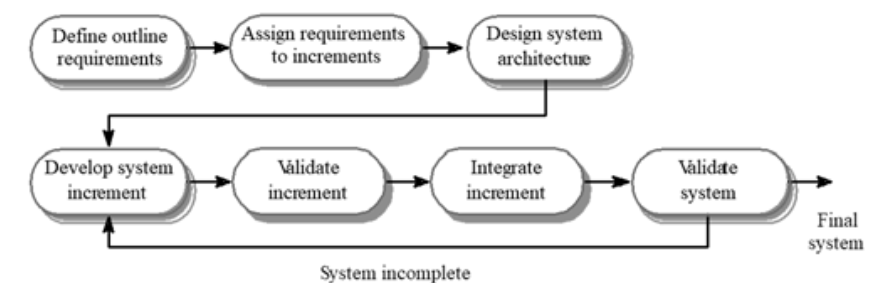
\includegraphics[width=0.7\textwidth]{./res/img/modello_incr.png}
			\caption{Rappresentazione del modello incrementale}
		\end{figure}
    Il modello incrementale é stato ritenuto preferibile considerando i seguenti vantaggi:
    \begin{itemize}
      \item ogni incremento porta un valore aggiunto, spingendo verso un'avanzamento continuo del progetto;
      \item sviluppo delle funzionalità più importanti all'inizio grazie all'ordinamento degli incrementi;
      \item i requisiti piú importanti vengono chiariti negli stadi iniziali della realizzazione del prodotto;
      \item l'uso di questo modello di sviluppo favorisce lo sviluppo di prototipi funzionanti, che a loro volta favoriscono la validazione dei requisiti e la comunicazione con il Proponente\ped{\textit{G}}.
    \end{itemize}

	\pagebreak
	
	\section{Pianificazione}
Lo sviluppo del progetto è costruito sulla base delle scadenze riportate nella sottosezione \textsection1.5 ed è suddiviso nelle seguenti fasi:
\begin{itemize}
	\item analisi;
	\item consolidamento dei requisiti
	\item progettazione architetturale;
	\item progettazione di dettaglio e codifica;
	\item validazione e collaudo.
\end{itemize}

\subsection{Analisi}
\textbf{Periodo}: dal 2020-03-10 al 2020-04-13 \\
Questo periodo ha inizio con la formazione dei gruppi e termina con la scadenza per la consegna dei documenti relativi alla \textit{Revisione dei Requisiti}. \\
Le principali attività svolte in questo periodo sono:
\begin{itemize}
	\item \textbf{Strumenti di lavoro}: questa attività consiste nella scelta degli strumenti di lavoro da utilizzare per lo svolgimento del progetto;
	\item \textbf{\NdP{}}: attività nella quale gli Amministratori redigono le \textit{\NdP{}}, documento in cui si specificano tutte le regole, le convenzioni e le tecnologie che i componenti del gruppo adotteranno durante tutto il corso del progetto. Questa attività include una stesura iniziale del documento, comprensiva delle norme e degli standard accordati dal gruppo, il documento verrà poi ampliato in base all'individuazione di sezioni da ampliare;
	\item \textbf{\SdF{}}: attività nella quale gli Analisti redigono lo \textit{\SdF}, documento in cui vengono analizzati i capitolati d'appalto elencando per ciascuno i punti positivi e negativi che li caratterizzano. Inoltre vengono indicate le motivazioni per le quali è stato scelto il capitolato\ped{\textit{G}} C2 denominato \textit{Etherless} e sono stati esclusi i capitolati restanti. \\
	Questa attività è bloccante per l'inizio dell'\textit{\AdR{}};
	\item \textbf{\AdR{}}: attività nella quale gli Analisti redigono l'\textit{\AdR{}}, documento essenziale in cui viene analizzato in maniera approfondita il capitolato\ped{\textit{G}} scelto a seguito dello \textit{\SdF}, individuando le funzionalità e i casi d'uso previsti dal progetto;
	\item \textbf{\PdP{}}: attività nella quale il Responsabile redige il \textit{\PdP}, documento in cui viene presentata la pianificazione del gruppo per lo sviluppo del progetto, un'analisi dei rischi e dei costi e dove vengono indicate le scadenze che il gruppo intende rispettare per la buona riuscita del progetto;
	\item \textbf{\PdQ{}}: attività nella quale gli Analisti redigono il \textit{\PdQ}, documento in cui vengono indicate tutte le strategie di verifica e validazione che il gruppo intende adottare con lo scopo di garantire la qualità di processo e di prodotto\ped{\textit{G}};
	\item \textbf{\Glossario{}}: attività nella quale viene redatto il \textit{\Glossario}, documento nel quale verranno elencati, chiariti ed approfonditi tutti i termini tecnici utilizzati nei documenti con lo scopo di evitare possibili ambiguità;
	\item \textbf{Lettera di Presentazione}: attività nella quale viene redatta la \textit{Lettera di Presentazione} necessaria per la presentazione come fornitore del gruppo.
\end{itemize}
	\subsubsection{Diagramma di Gantt: Analisi}
		\begin{figure}[h]
			\centering
			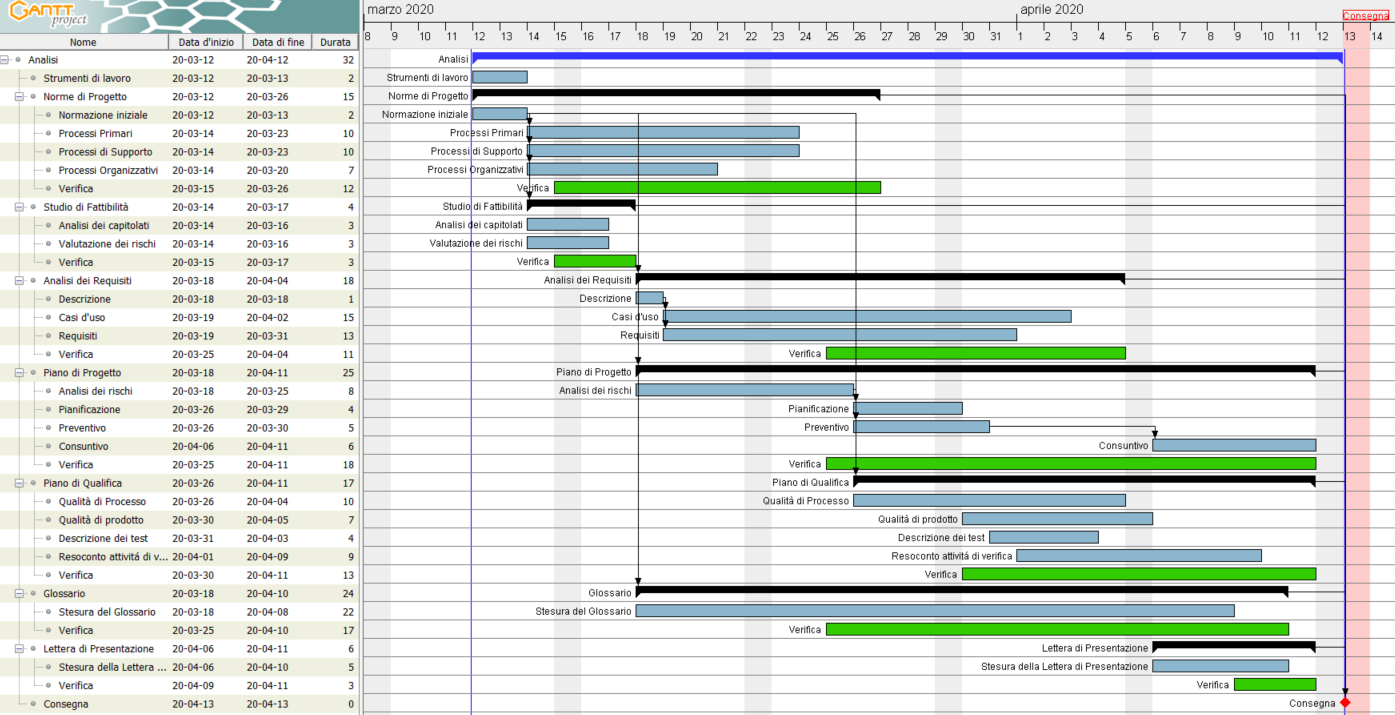
\includegraphics[width=1.1\textwidth]{./res/img/DiagrammiGantt/analisi_gantt.png}
			\caption{Diagramma di Gantt del periodo di Analisi}
		\end{figure}

\subsection{Consolidamento dei Requisiti}
\textbf{Periodo}: dal 2020-04-13 al 2020-04-20 \\
Questo periodo ha inizio dopo il termine del periodo di Analisi e termina il giorno della presentazione della \textit{Revisione dei Requisiti}. \\
\begin{itemize}
	\item \textbf{Incremento e Verifica dei documenti:} in caso di necessità, vengono migliorati e verificati i documenti preparati nel periodo precedente;
	\item \textbf{Consolidamento Analisi dei requisiti}: l'attività principale, prevede un consolidamento e un miglioramento dei requisiti ottenuti concluso il periodo di Analisi e conseguente aggiornamento dell'\textit{\AdR{}};
	\item \textbf{Realizzazione della presentazione:} preparazione del materiale necessario alla presentazione del 2020-04-20.
\end{itemize}
	\subsubsection{Diagramma di Gantt: Consolidamento dei Requisiti}
		\begin{figure}[h]
			\centering
			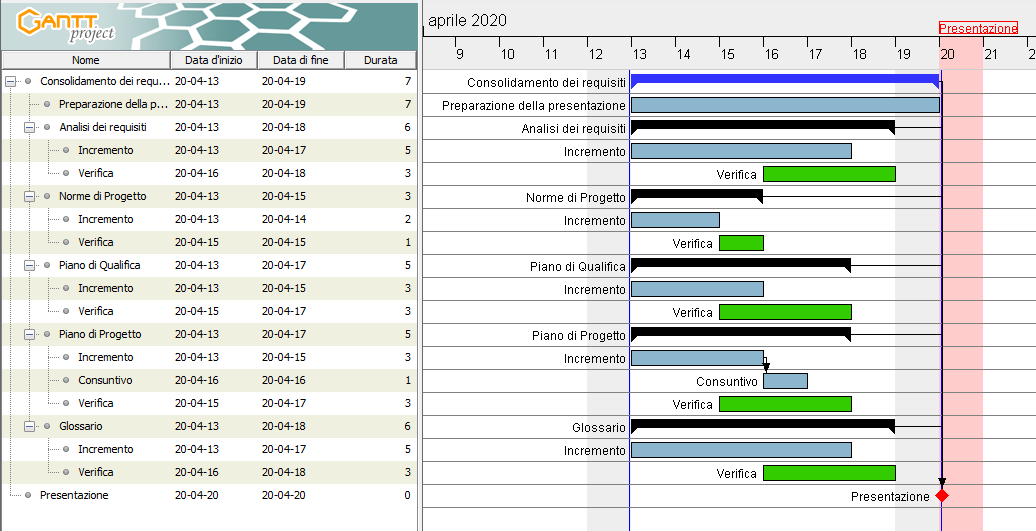
\includegraphics[width=1.1\textwidth]{./res/img/DiagrammiGantt/cons_req_gantt.png}
			\caption{Diagramma di Gantt del periodo di Consolidamento dei Requisiti}
		\end{figure}
\newpage
\subsection{Progettazione Architetturale}
\textbf{Periodo}: dal 2020-04-20 al 2020-05-11 \\
Questo periodo ha inizio al termine del periodo di Consolidamento dei Requisiti e termina con la scadenza per la consegna dei documenti relativi alla \textit{Revisione di Progettazione}. \\
Questo periodo porta all'individuazione di una soluzione architetturale che permetta il soddisfacimento dei requisiti individuati.
\begin{itemize}
	\item \textbf{Incremento e verifica}: come prima cosa, analizzando l'esito della \textit{Revisione dei Requisiti} vengono svolte attività di incremento e verifica sui vari documenti redatti, dove necessario. \\
	L'incremento dell'\textit{\AdR{}} è il più importante perchè va completato prima di poter proseguire con il resto delle attività;
	\item \textbf{Technology Baseline}: viene redatta la documentazione di supporto, contenente la descrizione delle tecnologie individuate e il tracciamento della relazione tra le componenti e i requisiti che vanno a soddisfare. Viene anche codificato il \textbf{PoC (Proof of Concept)} come dimostrazione del funzionamento dell'architettura individuata;
	\item \textbf{Glossario}: attività che prevede un miglioramento del \textit{Glossario} aggiungendo nuovi termini oppure raffinando le definizioni di termini già presenti.
\end{itemize}
	\subsubsection{Incrementi}
		\subsubsubsection{Descrizione}
			\begin{itemize}
				\item \textbf{1' Incremento:} integrazione dei documenti a seguito delle conoscenze acquisite nei periodi precedenti;
				\item \textbf{2' Incremento:} implementazione della componente Etherless\ped{\textit{G}}-smart;
				\item \textbf{3' Incremento:} implementazione della componenete Etherless\ped{\textit{G}}-cli; \\
				Comandi da implementare per il PoC:
					\begin{itemize}
						\item \textbf{signup:} legato allo UC3;
						\item \textbf{login:} legato allo UC5;
						\item \textbf{logout:} legato allo UC8;
						\item \textbf{run:} legato allo UC12.
					\end{itemize}
				\item \textbf{4' Incremento:} implementazione della componente Etherless\ped{\textit{G}}-server;
				\item \textbf{5' Incremento:} integrazione delle componenti sviluppate;
				\item \textbf{6' Incremento:} correzione della documentazione a seguito della correzione della RR e preparazione in vista della \TB{};
				\item \textbf{7' Incremento:} ulteriori aggiornamenti della documentazione;
				\begin{itemize}
					\item consuntivo di periodo nel \PdP{};
					\item aggiornamento \NdP{} e \PdQ{};
					\item eventuali aggiornamenti riguardanti il \Glossario{}.
				\end{itemize}
				\item \textbf{8' Incremento:} preparazione della presentazione per la RP.
			\end{itemize}
		\subsubsubsection{Scadenze}
			\begin{itemize}
				\item \textbf{1' Incremento:} entro 2020-04-22;
				\item \textbf{2' Incremento:} entro 2020-04-24;
				\item \textbf{3' Incremento:} entro 2020-04-26;
				\item \textbf{4' Incremento:} entro 2020-04-27;
				\item \textbf{5' Incremento:} entro 2020-04-28; % 29???
				\item \textbf{6' Incremento:} entro 2020-05-04;
				\item \textbf{7' Incremento:} entro 2020-05-11;
				\item \textbf{8' Incremento:} entro 2020-05-18.
			\end{itemize}

	\subsubsection{Diagramma di Gantt: Progettazione Architetturale}
		\begin{figure}[h]
			\centering
			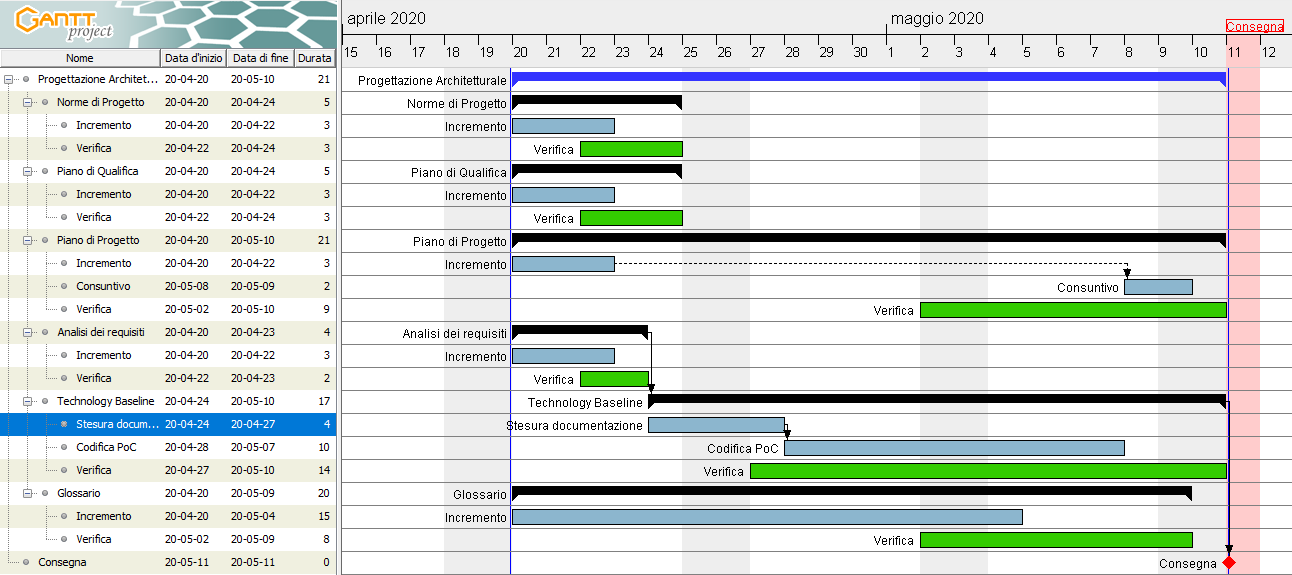
\includegraphics[width=1.1\textwidth]{./res/img/DiagrammiGantt/prog_arch_gantt.png}
			\caption{Diagramma di Gantt del periodo di Progettazione Architetturale}
		\end{figure}
\newpage
\subsection{Progettazione di Dettaglio e Codifica}
\textbf{Periodo}: dal 2020-05-11 al 2020-06-11 \\
Questo periodo ha inizio dopo il termine del periodo di Progettazione Architetturale, quindi alla scadenza della consegna della \textit{Revisione di Progettazione} e termina con la scadenza per la consegna dei documenti relativi alla \textit{Revisione di Qualifica}. \\
Le principali attività svolte in questo periodo sono:
\begin{itemize}
	\item \textbf{Incremento e verifica}: come prima cosa, analizzando l'esito della \textit{Revisione dei Progettazione} vengono svolte attività di incremento e verifica sui vari documenti redatti;
	\item \textbf{Product Baseline}: progettazione dettagliata a basso livello delle componenti del prodotto\ped{\textit{G}}, coerente con quanto individuato nella \TB{};
	\begin{itemize}
		\item \textbf{Allegato Tecnico}: stesura del documento di \textit{Allegato Tecnico}, di supporto alla progettazione di dettaglio;
		\item \textbf{Codifica}: attività nella quale viene prodotto\ped{\textit{G}} e verificato il codice.
	\end{itemize}
	\item \textbf{User Manual}(manuale utente): attività nella quale viene redatto lo \textit{User Manual} contenente le informazioni su come funziona e su come si utilizza il prodotto\ped{\textit{G}};
	\item \textbf{Glossario}: attività che prevede un miglioramento del \textit{Glossario} aggiungendo nuovi termini oppure raffinando le definizioni di termini già presenti.
\end{itemize}
	\subsubsection{Incrementi}
		\subsubsection{Descrizione}
			\begin{itemize}
				\item \textbf{1' Incremento:} correzione e integrazione dei documenti a seguito delle conoscenze acquisite nei periodi precedenti;
				\item \textbf{2' Incremento:} progettazione dei 3 moduli che compongono il sistema e stesura dell'\textit{Allegato Tecnico};
				\item \textbf{3' Incremento:} sviluppo di Etherless\ped{\textit{G}}-smart;
				\item \textbf{4' Incremento:} realizzazione delle componenti Etherless\ped{\textit{G}}-CLI e Etherless\ped{\textit{G}}-server (comprensivi di test di unitá e di integrazione);\\
				Comandi da implementare, legati ai requisiti obbligatori:
					\begin{itemize}
						\item \textbf{signup:} legato allo UC3;
						\item \textbf{login:} legato allo UC5;
						\item \textbf{logout:} legato allo UC8;
						\item \textbf{info:} legato allo UC10;
						\item \textbf{run:} legato allo UC12;
						\item \textbf{list:} legato agli UC13.1, UC13.1.1, UC13.3;
						\item \textbf{deploy:} legato allo UC14;
						\item \textbf{edit:} legato allo UC15;
						\item \textbf{delete:} legato allo UC18.
					\end{itemize}
				\item \textbf{5' Incremento:} ulteriori aggiornamenti della documentazione;% (consuntivo di periodo PdP e user manual)
					\begin{itemize}
						\item consuntivo di periodo nel \PdP{};
						\item stesura dello \textit{User Manual};
						\item aggiornamento dell' \textit{Allegato Tecnico};
						\item eventuali aggiornamenti riguardanti il \Glossario{}.
					\end{itemize}
				\item \textbf{6' Incremento:} preparazione della presentazione per la RQ.
			\end{itemize}
		\subsubsection{Scadenze}
			\begin{itemize}
				\item \textbf{1' Incremento:} entro 2020-05-20;
				\item \textbf{2' Incremento:} entro 2020-05-24;
				\item \textbf{3' Incremento:} entro 2020-05-26;
				\item \textbf{4' Incremento:} entro 2020-06-05;
				\item \textbf{5' Incremento:} entro 2020-06-11;
				\item \textbf{6' Incremento:} entro 2020-06-18.
			\end{itemize}
	\subsubsection{Diagramma di Gantt: Progettazione di Dettaglio e Codifica}
		\begin{figure}[h]
			\centering
			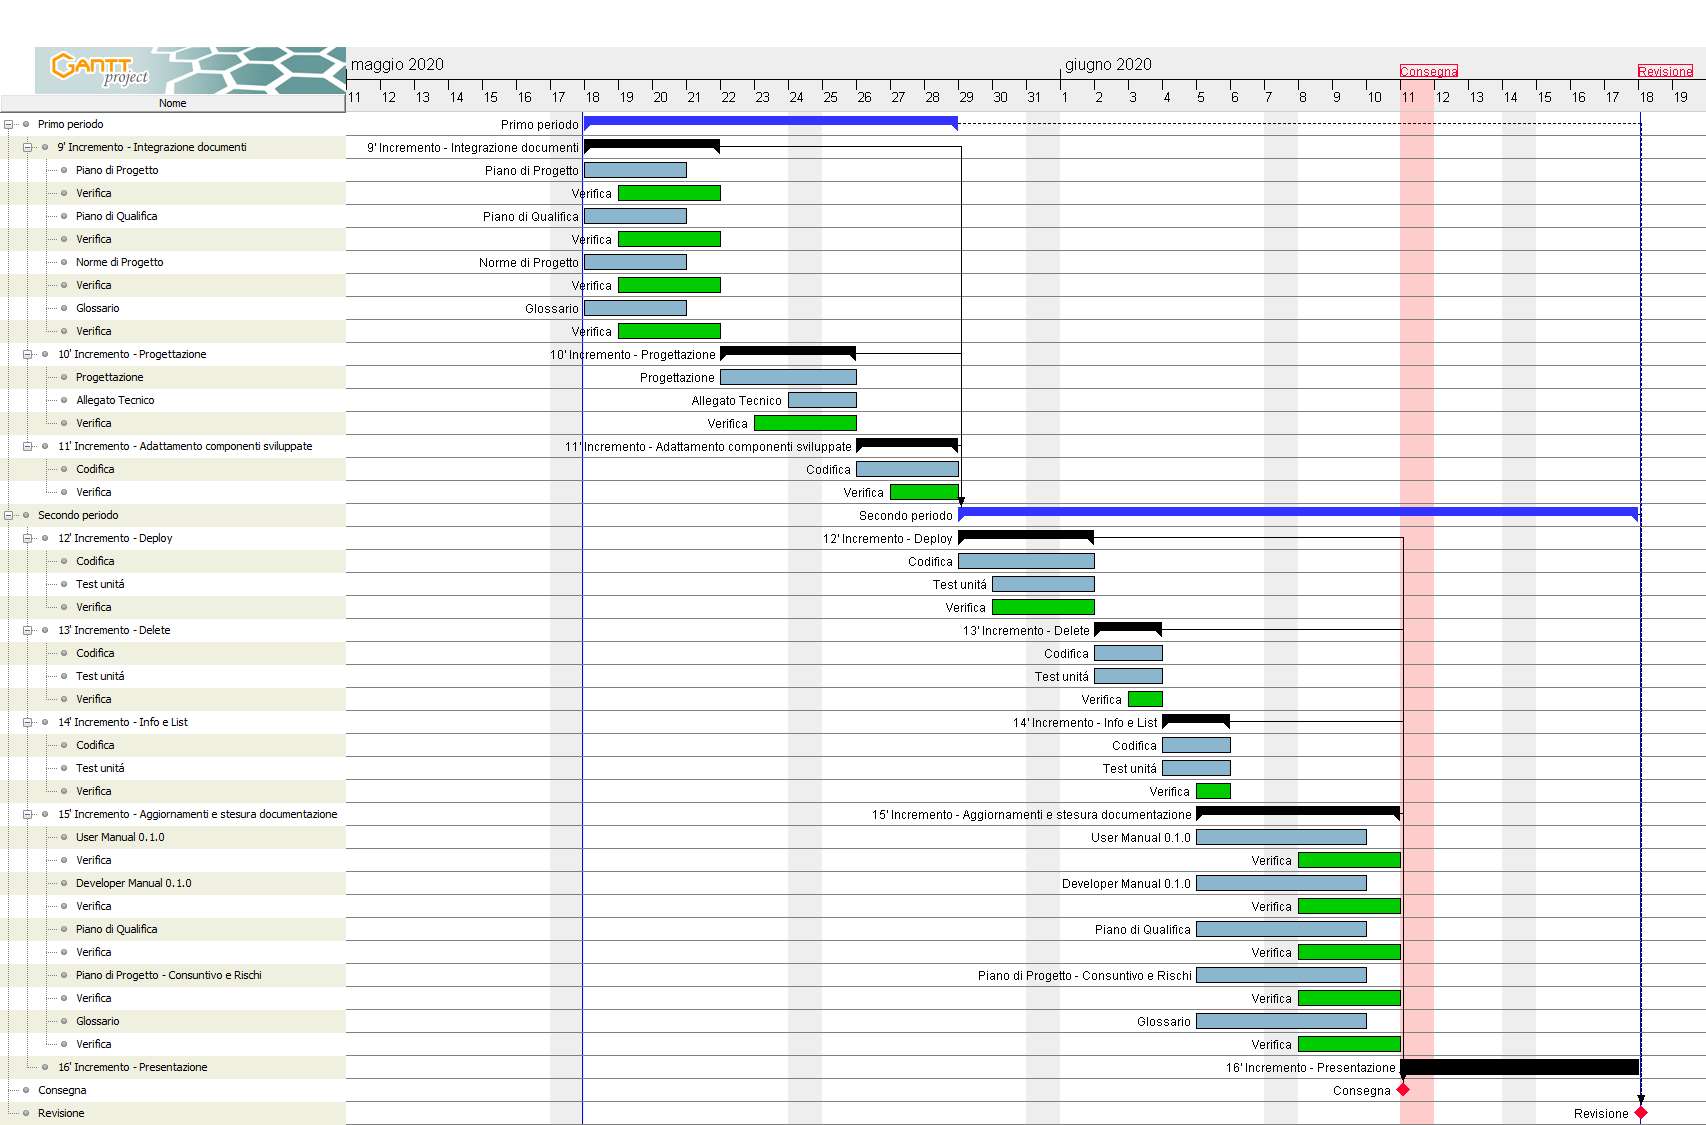
\includegraphics[width=1.1\textwidth]{./res/img/DiagrammiGantt/prog_dett_gantt.png}
			\caption{Diagramma di Gantt del periodo di Progettazione di Dettaglio e Codifica}
		\end{figure}
\newpage
\subsection{Validazione e Collaudo}
\textbf{Periodo}: dal 2020-06-11 al 2020-07-13 \\
Questo periodo ha inizio dopo il termine del periodo di Progettazione di Dettaglio e Codifica e termina con la scadenza per la consegna dei documenti relativi alla \textit{Revisione di Accettazione}. \\
Le principali attività svolte in questo periodo sono:
\begin{itemize}
	\item \textbf{Incremento e verifica}: come prima cosa, analizzando l'esito della \textit{Revisione dei Qualifica} vengono svolte attività di incremento e verifica sui vari documenti redatti;
	\item \textbf{Validazione e Collaudo}: attività nella quale vengono eseguiti test e, se necessario, vengono apportati dei miglioramenti al prodotto\ped{\textit{G}} per poter assicurare il soddisfacimento dei requisiti e dei vincoli qualitativi;
	\item \textbf{User Manual}: attività nella quale viene migliorato lo \textit{User Manual};
	\item \textbf{Manuale Sviluppatore}: attività nella quale viene redatto il \textit{Manuale Sviluppatore}, il quale contiene le informazioni utili al mantenimento del prodotto\ped{\textit{G}};
	\item \textbf{Glossario}: attività che prevede un miglioramento del \textit{Glossario} aggiungendo nuovi termini oppure raffinando le definizioni di termini già presenti.
\end{itemize}
	\subsubsection{Incrementi}
		\subsubsubsection{Descrizione}
			\begin{itemize}
				\item \textbf{1' Incremento:} correzione e integrazione dei documenti a seguito delle conoscenze acquisite nei periodi precedenti e dalla correzione della RQ;
				\item \textbf{2' Incremento:} implementazione dei requisiti mancanti, ovvero quelli desiderabili e opzionali;\\
				Comandi da implementare, legati a requisiti desiderabili e opzionali:
					\begin{itemize}
						\item \textbf{init};
						\item \textbf{help:} legato a UC1 e UC2;
						\item \textbf{whoami:} legato allo UC9;
						\item \textbf{search:} legato allo UC11;
						\item \textbf{history:} legato allo UC16.
					\end{itemize}
				\item \textbf{2' Incremento:} implementazione dei test di sistema ed eventuali correzioni necessarie;
				\item \textbf{4' Incremento:} aggiornamento dei documenti e stesura del \textit{Manuale dello Sviluppatore};
				\item \textbf{5' Incremento:} preparazione della presentazione per la RA.
			\end{itemize}
		\subsubsubsection{Scadenze}
			\begin{itemize}
				\item \textbf{1' Incremento:} entro 2020-06-26;
				\item \textbf{2' Incremento:} entro 2020-07-02;
				\item \textbf{3' Incremento:} entro 2020-07-08;
				\item \textbf{4' Incremento:} entro 2020-07-13;
				\item \textbf{5' Incremento:} entro 2020-07-20.
			\end{itemize}
	\subsubsection{Diagramma di Gantt: Validazione e Collaudo}
		\begin{figure}[h]
			\centering
			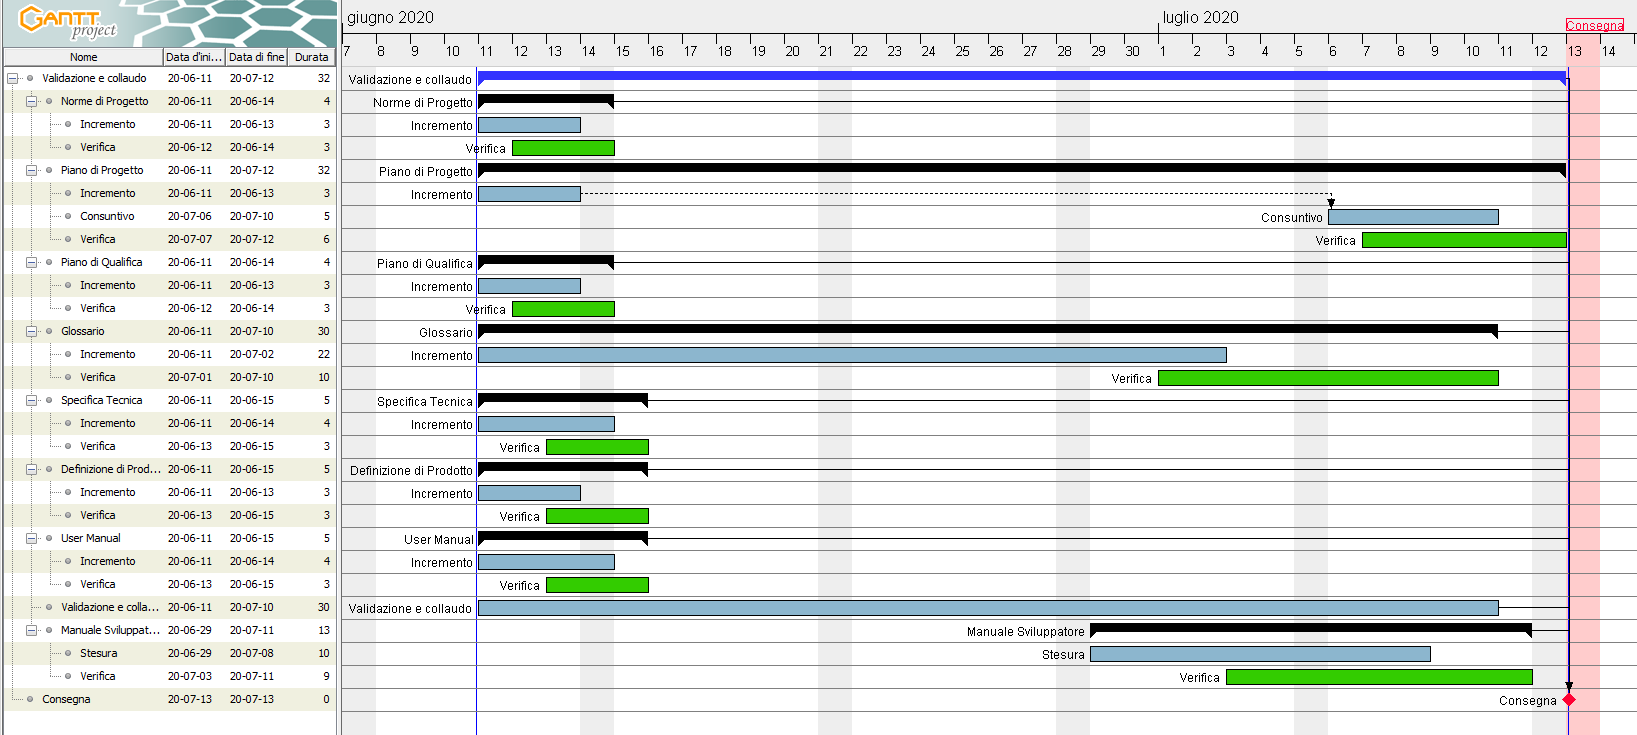
\includegraphics[width=1.1\textwidth]{./res/img/DiagrammiGantt/validaz_gantt.png}
			\caption{Diagramma di Gantt del periodo di Validazione e Collaudo}
		\end{figure}

	\pagebreak
	
	\section{Preventivo}
È importante tener conto che i periodi di Analisi e Consolidamento dei requisiti sono considerati un investimento per il gruppo e che quindi non sono a carico del Committente\ped{\textit{G}}.
Di conseguenza le ore necessarie allo svolgimento delle attività di questi due periodi saranno conteggiate nel totale delle ore da retribuire. \\

La suddivisione oraria viene fatta rispettando le seguenti regole:
\begin{itemize}
	\item il totale delle ore di lavoro deve essere equamente distribuito tra i componenti del gruppo;
	\item ciascun componente deve ricoprire ogni ruolo almeno una volta;
	\item non si dovranno verificare situazioni nelle quali un Verificatore debba verificare il proprio lavoro.
\end{itemize}

Per semplificare la lettura delle tabelle seguenti verranno utilizzate le seguenti sigle per identificare i ruoli:
\begin{itemize}
	\item \textbf{Rp}: Responsabile di Progetto;
	\item \textbf{As}: Amministratore;
	\item \textbf{An}: Analista;
	\item \textbf{Pt}: Progettista;
	\item \textbf{Pr}: Programmatore;
	\item \textbf{Vf}: Verificatore.
\end{itemize}
Inoltre le celle che contengono un valore pari a 0 presenteranno il simbolo '-'.

\newpage

\subsection{Analisi}
	\subsubsection{Prospetto orario}
		Distribuzione delle ore per ciascun ruolo nel periodo di Analisi:

		\rowcolors{2}{lightRowColor}{darkRowColor}
		\begin{longtable}{
			>{\centering}p{0.25\textwidth}
			>{\centering}p{0.05\textwidth}
			>{\centering}p{0.05\textwidth}
			>{\centering}p{0.05\textwidth}
			>{\centering}p{0.05\textwidth}
			>{\centering}p{0.05\textwidth}
			>{\centering}p{0.05\textwidth}
			>{\centering\arraybackslash}p{0.15\textwidth} }

			\coloredTableHead
			\textbf{\color{white}Nome} &
			\textbf{\color{white}Rp} &
			\textbf{\color{white}As} &
			\textbf{\color{white}An} &
			\textbf{\color{white}Pt} &
			\textbf{\color{white}Pr} &
			\textbf{\color{white}Vf} &
			\textbf{\color{white}Totale}
			\tabularnewline
			\endhead

			% Contenuto della tabella
			% Nome & Rp & As & An & Pt & Pr & Vf & Totale \\
			\VB & 10 & 20 & -  & -  & - & -  & 30 \\
			\LB & -  & 20 & -  & -  & - & 10 & 30 \\
			\NF & -  & 20 & -  & 10 & - & -  & 30 \\
			\EG & -  & 5  & 30 & -  & - & -  & 35 \\
			\FJ & -  & -  & -  & 10 & - & 20 & 30 \\
			\MP & 20 & -  & -  & -  & - & 10 & 30 \\
			\AS & -  & 5  & -  & -  & - & 25 & 30 \\
			\AZ & -  & -  & 30 & -  & - & 5  & 35 \\
			\textbf{Ore totali per ruolo} & 30 & 70 & 60 & 20 & - & 70 & 250 \\

			\rowcolor{white}\caption{Suddivisione oraria del periodo di Analisi}	\\

		\end{longtable}

		% Grafico
		Rappresentazione grafica della suddivisione oraria:
		\begin{figure}[h]
			\centering
			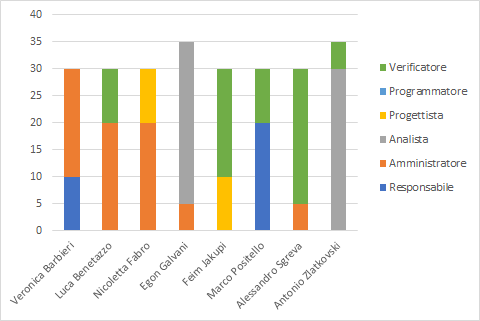
\includegraphics[width=0.7\textwidth]{./res/img/analisi_po.png}
			\caption{Suddivisione oraria del periodo di Analisi}
		\end{figure}

	\newpage
	\subsubsection{Prospetto economico}
		Totale delle ore e costo per ciascun ruolo nel periodo di Analisi:

		\rowcolors{2}{lightRowColor}{darkRowColor}
		\begin{longtable}{
			>{\centering}p{0.25\textwidth}
			>{\centering}p{0.05\textwidth}
			>{\centering\arraybackslash}p{0.15\textwidth} }

			\coloredTableHead
			\textbf{\color{white}Ruolo} &
			\textbf{\color{white}Ore} &
			\textbf{\color{white}Costo in \euro{}}
			\tabularnewline
			\endhead

			% Contenuto della tabella
			% Ruolo & Ore & Costo\\
			Responsabile    & 30  & 900,00 \\
			Amministratore  & 70  & 1.400,00 \\
			Analista        & 60  & 1.500,00 \\
			Progettista     & 20  & 440,00 \\
			Programmatore   & -   & - \\
			Verificatore    & 70  & 1.050,00 \\
			\textbf{Totale} & 250 & 5.290,00 \\

			\rowcolor{white}\caption{Prospetto dei costi per il periodo di Analisi}	\\

		\end{longtable}

		% Grafico
		Rappresentazione grafica della distribuzione dei ruoli:
		\begin{figure}[h]
			\centering
			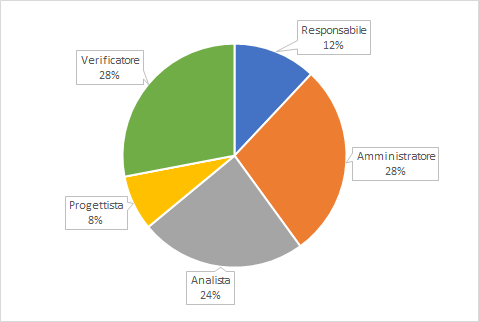
\includegraphics[width=0.7\textwidth]{./res/img/analisi_pe.png}
			\caption{Suddivisione dei ruoli nel periodo di Analisi}
		\end{figure}

\newpage
\subsection{Consolidamento dei Requisiti}
	\subsubsection{Prospetto orario}
		Distribuzione delle ore per ciascun ruolo nel periodo di Consolidamento dei requisiti:

		\rowcolors{2}{lightRowColor}{darkRowColor}
		\begin{longtable}{
			>{\centering}p{0.25\textwidth}
			>{\centering}p{0.05\textwidth}
			>{\centering}p{0.05\textwidth}
			>{\centering}p{0.05\textwidth}
			>{\centering}p{0.05\textwidth}
			>{\centering}p{0.05\textwidth}
			>{\centering}p{0.05\textwidth}
			>{\centering\arraybackslash}p{0.15\textwidth} }

			\coloredTableHead
			\textbf{\color{white}Nome} &
			\textbf{\color{white}Rp} &
			\textbf{\color{white}As} &
			\textbf{\color{white}An} &
			\textbf{\color{white}Pt} &
			\textbf{\color{white}Pr} &
			\textbf{\color{white}Vf} &
			\textbf{\color{white}Totale}
			\tabularnewline
			\endhead

			% Contenuto della tabella
			% Nome & Rp & As & An & Pt & Pr & Vf & Totale \\
			\VB & - & - & 3 & - & - & 2 & 5 \\
			\LB & 5 & - & - & - & - & - & 5 \\
			\NF & - & - & - & - & - & 5 & 5 \\
			\EG & - & 3 & - & - & - & - & 3 \\
			\FJ & - & - & 3 & - & - & 2 & 5 \\
			\MP & - & - & 2 & - & - & 3 & 5 \\
			\AS & - & - & 2 & - & - & 3 & 5 \\
			\AZ & - & 3 & - & - & - & - & 3 \\
			\textbf{Ore totali per ruolo} & 5 & 6 & 10 & - & - & 15 & 36 \\

			\rowcolor{white}\caption {Suddivisione oraria del periodo di Consolidamento dei requisiti} \\

		\end{longtable}

		% Grafico
		Rappresentazione grafica della suddivisione oraria:
		\begin{figure}[h]
			\centering
			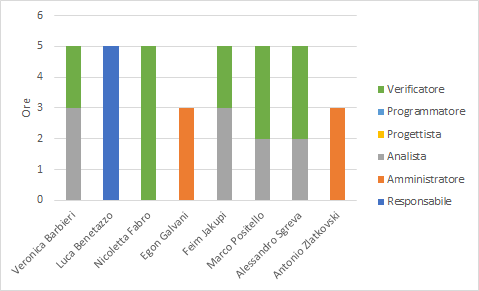
\includegraphics[width=0.7\textwidth]{./res/img/consolidamentoRequisiti_po.png}
			\caption{Suddivisione oraria del periodo di Consolidamento dei requisiti}
		\end{figure}

	\newpage
	\subsubsection{Prospetto economico}
		Totale delle ore e costo per ciascun ruolo nel periodo di Consolidamento dei requisiti:

		\rowcolors{2}{lightRowColor}{darkRowColor}
		\begin{longtable}{
			>{\centering}p{0.25\textwidth}
			>{\centering}p{0.05\textwidth}
			>{\centering\arraybackslash}p{0.15\textwidth} }

			\coloredTableHead
			\textbf{\color{white}Ruolo} &
			\textbf{\color{white}Ore} &
			\textbf{\color{white}Costo in \euro{}}
			\tabularnewline
			\endhead

			% Contenuto della tabella
			% Ruolo & Ore & Costo \\
			Responsabile    & 5  & 150,00 \\
			Amministratore  & 6  & 120,00 \\
			Analista        & 10 & 250,00 \\
			Progettista     & -  & - \\
			Programmatore   & -  & - \\
			Verificatore    & 15 & 225,00 \\
			\textbf{Totale} & 36 & 745,00 \\

			\rowcolor{white}\caption {Prospetto dei costi per il periodo di Consolidamento dei requisiti}	\\

		\end{longtable}

		% Grafico
		Rappresentazione grafica della distribuzione dei ruoli:
		\begin{figure}[h]
			\centering
			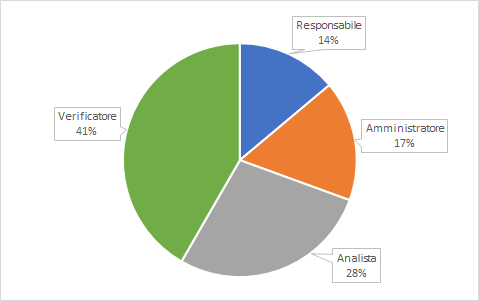
\includegraphics[width=0.7\textwidth]{./res/img/consolidamentoRequisiti_pe.png}
			\caption{Suddivisione dei ruoli nel periodo di Consolidamento dei requisiti}
		\end{figure}

\newpage
\subsection{Progettazione Architetturale}
	\subsubsection{Prospetto orario}
		Distribuzione delle ore per ciascun ruolo nel periodo di Progettazione architetturale:

		\rowcolors{2}{lightRowColor}{darkRowColor}
		\begin{longtable}{
			>{\centering}p{0.25\textwidth}
			>{\centering}p{0.05\textwidth}
			>{\centering}p{0.05\textwidth}
			>{\centering}p{0.05\textwidth}
			>{\centering}p{0.05\textwidth}
			>{\centering}p{0.05\textwidth}
			>{\centering}p{0.05\textwidth}
			>{\centering\arraybackslash}p{0.15\textwidth} }

			\coloredTableHead
			\textbf{\color{white}Nome} &
			\textbf{\color{white}Rp} &
			\textbf{\color{white}As} &
			\textbf{\color{white}An} &
			\textbf{\color{white}Pt} &
			\textbf{\color{white}Pr} &
			\textbf{\color{white}Vf} &
			\textbf{\color{white}Totale}
			\tabularnewline
			\endhead

			% Contenuto della tabella
			% Nome & Rp & As & An & Pt & Pr & Vf & Totale \\
			\VB & - & -  & -  & 8  & 7 & 16 & 31 \\
			\LB & 5 & -  & 10 & 11 & 5 & -  & 31 \\
			\NF & - & -  & 6  & 15 & - & 10 & 31 \\
			\EG & - & -  & 7  & 8  & 6 & 10 & 31 \\
			\FJ & - & 6  & -  & 8  & 7 & 10 & 31 \\
			\MP & - & 8  & -  & 15 & - & 8  & 31 \\
			\AS & - & 10 & -  & 7  & 6 & 8  & 31 \\
			\AZ & 7 & -  & 10 & -  & 8 & 6  & 31 \\
			\textbf{Ore totali per ruolo} & 12 & 24 & 33 & 72 & 39 & 68 & 248 \\

			\rowcolor{white}\caption {Suddivisione oraria del periodo di Progettazione architetturale} \\

		\end{longtable}

		% Grafico
		\begin{figure}[h]
			\centering
			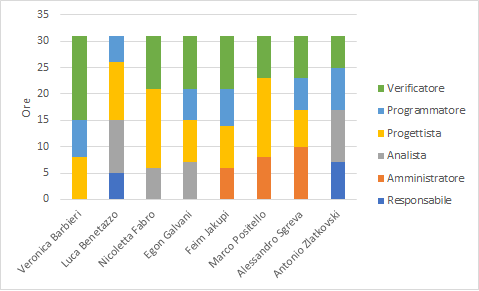
\includegraphics[width=0.7\textwidth]{./res/img/progettazioneArchitetturale_po.png}
			\caption{Suddivisione oraria del periodo di Progettazione architetturale}
		\end{figure}

		\newpage
		\subsubsection{Pianificazione oraria interna agli incrementi}
		\rowcolors{2}{lightRowColor}{darkRowColor}
		\begin{longtable}{
			>{\centering}p{0.25\textwidth}
			>{\centering}p{0.05\textwidth}
			>{\centering}p{0.05\textwidth}
			>{\centering}p{0.05\textwidth}
			>{\centering}p{0.05\textwidth}
			>{\centering}p{0.05\textwidth}
			>{\centering}p{0.05\textwidth}
			>{\centering\arraybackslash}p{0.10\textwidth}
			>{\centering\arraybackslash}p{0.10\textwidth} }

			\coloredTableHead
			\textbf{\color{white}Incremento} &
			\textbf{\color{white}Rp} &
			\textbf{\color{white}As} &
			\textbf{\color{white}An} &
			\textbf{\color{white}Pt} &
			\textbf{\color{white}Pr} &
			\textbf{\color{white}Vf} &
			\textbf{\color{white}Totale ore} &
			\textbf{\color{white}Totale \euro{}}
			\tabularnewline
			\endhead

			% Contenuto della tabella
			% n'Incr & Rp & As & An & Pt & Pr & Vf & Totale Ore \\
			1' Incremento & 2 & 5  & 11 & 7  & -  & 11 & 35 & 754,00\\
			2' Incremento & 1 & 5  & 8  & 12 & 9  & 8  & 43 & 849,00\\
			3' Incremento & 1 & 3  & 3  & 14 & 10 & 8  & 39 & 743,00\\
			4' Incremento & 1 & 3  & 3  & 14 & 10 & 8  & 39 & 743,00\\
			5' Incremento & 2 & 3  & 3  & 12 & 10 & 7  & 37 & 714,00\\
			6' Incremento & 2 & 3  & 4  & 7  & -  & 13 & 29 & 569,00\\
			7' Incremento & 2 & 1  & 1  & 6  & -  & 11 & 21 & 402,00\\
			8' Incremento & 1 & 1  & -  & -  & -  & 2  & 4  & 80,00\\
			\textbf{Ore e costo totali} & 12 & 24 & 33 & 72 & 39 & 68 & 248 & 4.854,00 \\

			\rowcolor{white}\caption {Suddivisione oraria per incremento del periodo di Progettazione architetturale} \\

		\end{longtable}

	\subsubsection{Prospetto economico}
		Totale delle ore e costo per ciascun ruolo nel periodo di Progettazione architetturale:

		\rowcolors{2}{lightRowColor}{darkRowColor}
		\begin{longtable}{
			>{\centering}p{0.25\textwidth}
			>{\centering}p{0.05\textwidth}
			>{\centering\arraybackslash}p{0.15\textwidth} }

			\coloredTableHead
			\textbf{\color{white}Ruolo} &
			\textbf{\color{white}Ore} &
			\textbf{\color{white}Costo in \euro{}}
			\tabularnewline
			\endhead

			% Contenuto della tabella
			% Ruolo & Ore & Costo \\
			Responsabile    & 12  & 360,00 \\
			Amministratore  & 24  & 480,00 \\
			Analista        & 33  & 825,00 \\
			Progettista     & 72  & 1.584,00 \\
			Programmatore   & 39  & 585,00 \\
			Verificatore    & 68  & 1.020,00 \\
			\textbf{Totale} & 248 & 4.854,00 \\

			\rowcolor{white}\caption {Prospetto dei costi per il periodo di Progettazione architetturale}	\\

		\end{longtable}

		% Grafico
		Rappresentazione grafica della distribuzione dei ruoli:
		\begin{figure}[h]
			\centering
			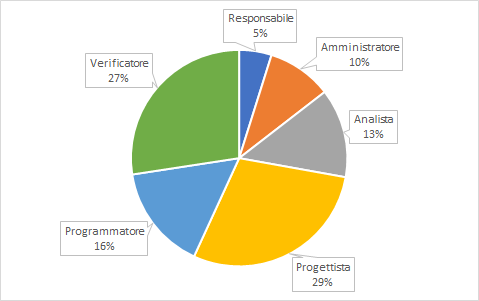
\includegraphics[width=0.7\textwidth]{./res/img/progettazioneArchitetturale_pe.png}
			\caption{Suddivisione dei ruoli nel periodo di Progettazione architetturale}
		\end{figure}

\newpage
\subsection{Progettazione di Dettaglio e Codifica}
	\subsubsection{Prospetto orario}
	Distribuzione delle ore per ciascun ruolo nel periodo di Progettazione di dettaglio e codifica:

		\rowcolors{2}{lightRowColor}{darkRowColor}
		\begin{longtable}{
			>{\centering}p{0.25\textwidth}
			>{\centering}p{0.05\textwidth}
			>{\centering}p{0.05\textwidth}
			>{\centering}p{0.05\textwidth}
			>{\centering}p{0.05\textwidth}
			>{\centering}p{0.05\textwidth}
			>{\centering}p{0.05\textwidth}
			>{\centering\arraybackslash}p{0.15\textwidth} }

			\coloredTableHead
			\textbf{\color{white}Nome} &
			\textbf{\color{white}Rp} &
			\textbf{\color{white}As} &
			\textbf{\color{white}An} &
			\textbf{\color{white}Pt} &
			\textbf{\color{white}Pr} &
			\textbf{\color{white}Vf} &
			\textbf{\color{white}Totale}
			\tabularnewline
			\endhead

			% Contenuto della tabella
			% Nome & Rp & As & An & Pt & Pr & Vf & Totale \\
			\VB & 7 & 4 & - & 6  & 20 & 12 & 49 \\
			\LB & - & - & - & 15 & 20 & 14 & 49 \\
			\NF & - & 8 & - & 12 & 19 & 10 & 49 \\
			\EG & 6 & - & - & 15 & 20 & 8  & 49 \\
			\FJ & 5 & 5 & - & 10 & 19 & 10 & 49 \\
			\MP & 5 & 6 & - & 8  & 15 & 15 & 49 \\
			\AS & - & - & - & 14 & 20 & 15 & 49 \\
			\AZ & - & 9 & - & 8  & 20 & 12 & 49 \\
			\textbf{Ore totali per ruolo} & 23 & 32 & - & 88 & 153 & 96 & 392 \\

			\rowcolor{white}\caption {Suddivisione oraria del periodo di Progettazione di dettaglio e codifica} \\

		\end{longtable}

		\newpage
		% Grafico
		Rappresentazione grafica della suddivisione oraria:
		\begin{figure}[h]
			\centering
			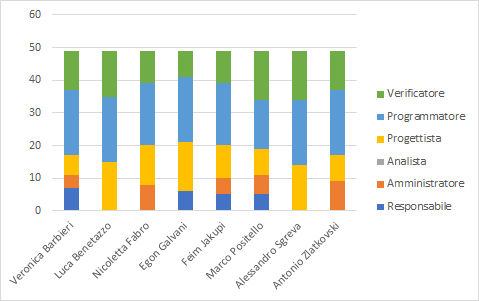
\includegraphics[width=0.7\textwidth]{./res/img/progettazioneDettaglioCodifica_po.png}
			\caption{Suddivisione oraria del periodo di Progettazione di dettaglio e codifica}
		\end{figure}

		\subsubsection{Pianificazione oraria interna agli incrementi}
		\rowcolors{2}{lightRowColor}{darkRowColor}
		\begin{longtable}{
			>{\centering}p{0.25\textwidth}
			>{\centering}p{0.05\textwidth}
			>{\centering}p{0.05\textwidth}
			>{\centering}p{0.05\textwidth}
			>{\centering}p{0.05\textwidth}
			>{\centering}p{0.05\textwidth}
			>{\centering}p{0.05\textwidth}
			>{\centering\arraybackslash}p{0.10\textwidth}
			>{\centering\arraybackslash}p{0.10\textwidth} }

			\coloredTableHead
			\textbf{\color{white}Incremento} &
			\textbf{\color{white}Rp} &
			\textbf{\color{white}As} &
			\textbf{\color{white}An} &
			\textbf{\color{white}Pt} &
			\textbf{\color{white}Pr} &
			\textbf{\color{white}Vf} &
			\textbf{\color{white}Totale ore} &
			\textbf{\color{white}Totale \euro{}}
			\tabularnewline
			\endhead

			% Contenuto della tabella
			% n'Incr & Rp & As & An & Pt & Pr & Vf & Totale Ore \\
			1' Incremento & 2 & 8 & - & 10 & -  & 17 & 37 & 695,00\\
			2' Incremento & 6 & 4 & - & 35 & 27 & 25 & 97 & 1.810,00\\
			3' Incremento & 5 & 7 & - & 15 & 50 & 15 & 92 & 1.595,00\\
			4' Incremento & 5 & 7 & - & 23 & 75 & 30 & 39 & 2.371,00\\
			5' Incremento & 3 & 4 & - & 3  & 1  & 1  & 16 & 319,00\\
			6' Incremento & 2 & 2 & - & 3  & 1  & 1  & 10 & 211,00\\
			\textbf{Ore e costo totali} & 23 & 32 & - & 88 & 153 & 96 & 392 & 7.001,00 \\

			\rowcolor{white}\caption {Suddivisione oraria per incremento del periodo di Progettazione di Dettaglio e Codifica} \\

		\end{longtable}

	\newpage
	\subsubsection{Prospetto economico}
		Totale delle ore e costo per ciascun ruolo nel periodo di Progettazione di dettaglio e codifica:

		\rowcolors{2}{lightRowColor}{darkRowColor}
		\begin{longtable}{
			>{\centering}p{0.25\textwidth}
			>{\centering}p{0.05\textwidth}
			>{\centering\arraybackslash}p{0.15\textwidth} }

			\coloredTableHead
			\textbf{\color{white}Ruolo} &
			\textbf{\color{white}Ore} &
			\textbf{\color{white}Costo in \euro{}}
			\tabularnewline
			\endhead

			% Contenuto della tabella
			% Ruolo & Ore & Costo \\
			Responsabile    & 23 & 690,00 \\
			Amministratore  & 32 & 640,00 \\
			Analista        & -  & - \\
			Progettista     & 88 & 1.936,00 \\
			Programmatore   & 153 & 2.295,00 \\
			Verificatore    & 96  & 1.440,00 \\
			\textbf{Totale} & 392 & 7.001,00 \\

			\rowcolor{white}\caption {Prospetto dei costi per il periodo di Progettazione di dettaglio e codifica} \\

		\end{longtable}

		% Grafico
		Rappresentazione grafica della distribuzione dei ruoli:
		\begin{figure}[h]
			\centering
			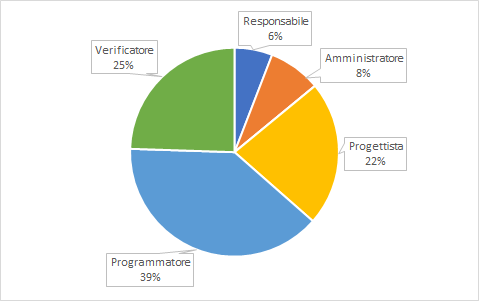
\includegraphics[width=0.7\textwidth]{./res/img/progettazioneDettaglioCodifica_pe.png}
			\caption{Suddivisione dei ruoli nel periodo di Progettazione di dettaglio e codifica}
		\end{figure}

\newpage
\subsection{Validazione e Collaudo}
	\subsubsection{Prospetto orario}
	Distribuzione delle ore per ciascun ruolo nel periodo di Validazione e collaudo:

		\rowcolors{2}{lightRowColor}{darkRowColor}
		\begin{longtable}{
			>{\centering}p{0.25\textwidth}
			>{\centering}p{0.05\textwidth}
			>{\centering}p{0.05\textwidth}
			>{\centering}p{0.05\textwidth}
			>{\centering}p{0.05\textwidth}
			>{\centering}p{0.05\textwidth}
			>{\centering}p{0.05\textwidth}
			>{\centering\arraybackslash}p{0.15\textwidth} }

			\coloredTableHead
			\textbf{\color{white}Nome} &
			\textbf{\color{white}Rp} &
			\textbf{\color{white}As} &
			\textbf{\color{white}An} &
			\textbf{\color{white}Pt} &
			\textbf{\color{white}Pr} &
			\textbf{\color{white}Vf} &
			\textbf{\color{white}Totale}
			\tabularnewline
			\endhead

			% Contenuto della tabella
			% Nome & Rp & As & An & Pt & Pr & Vf & Totale \\
			\VB & - & - & - & 5 & 7  & 10 & 22 \\
			\LB & - & 6 & - & - & 10 & 6  & 22 \\
			\NF & 5 & - & - & - & 7  & 10 & 22 \\
			\EG & - & 5 & - & 7 & -  & 10 & 22 \\
			\FJ & 6 & 6 & - & - & 5  & 5  & 22 \\
			\MP & 5 & - & - & - & 7  & 10 & 22 \\
			\AS & 6 & - & - & - & 5  & 11 & 22 \\
			\AZ & - & - & - & 6 & 6  & 10 & 22 \\
			\textbf{Ore totali per ruolo} & 22 & 17 & - & 18 & 47 & 72 & 176 \\

			\rowcolor{white}\caption {Suddivisione oraria del periodo di Validazione e collaudo} \\

		\end{longtable}

		% Grafico
		Rappresentazione grafica della suddivisione oraria:
		\begin{figure}[h]
			\centering
			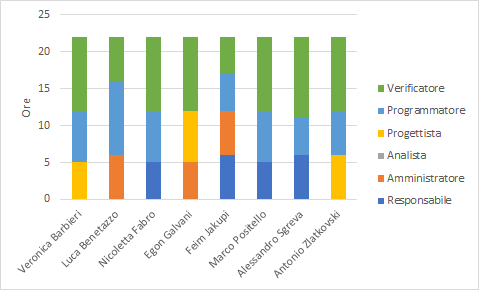
\includegraphics[width=0.7\textwidth]{./res/img/validazioneCollaudo_po.png}
			\caption{Suddivisione oraria del periodo di Validazione e collaudo}
		\end{figure}

		\newpage
		\subsubsection{Pianificazione oraria interna agli incrementi}
		\rowcolors{2}{lightRowColor}{darkRowColor}
		\begin{longtable}{
			>{\centering}p{0.25\textwidth}
			>{\centering}p{0.05\textwidth}
			>{\centering}p{0.05\textwidth}
			>{\centering}p{0.05\textwidth}
			>{\centering}p{0.05\textwidth}
			>{\centering}p{0.05\textwidth}
			>{\centering}p{0.05\textwidth}
			>{\centering\arraybackslash}p{0.10\textwidth}
			>{\centering\arraybackslash}p{0.10\textwidth} }

			\coloredTableHead
			\textbf{\color{white}Incremento} &
			\textbf{\color{white}Rp} &
			\textbf{\color{white}As} &
			\textbf{\color{white}An} &
			\textbf{\color{white}Pt} &
			\textbf{\color{white}Pr} &
			\textbf{\color{white}Vf} &
			\textbf{\color{white}Totale ore} &
			\textbf{\color{white}Totale \euro{}}
			\tabularnewline
			\endhead

			% Contenuto della tabella
			% n'Incr & Rp & As & An & Pt & Pr & Vf & Totale Ore \\
			1' Incremento & 7 & 6 & - & 3 & 5 & 9 & 30 & 606,00\\
			2' Incremento & 3 & 3 & - & 7 & 23 & 25 & 61 & 1.024,00\\
			3' Incremento & 3 & 3 & - & 4 & 16 & 22 & 48 & 808,00\\
			4' Incremento & 7 & 4 & - & 3 & 2 & 14 & 30 & 596,00\\
			5' Incremento & 2 & 1 & - & 1 & 1 & 2 & 7 & 147,00\\
			\textbf{Ore e costo totali} & 22 & 17 & - & 18 & 47 & 72 & 176 & 3.181,00 \\

			\rowcolor{white}\caption {Suddivisione oraria per incremento del periodo di Validazione e collaudo} \\

		\end{longtable}

	\subsubsection{Prospetto economico}
		Totale delle ore e costo per ciascun ruolo nel periodo di Validazione e collaudo:

		\rowcolors{2}{lightRowColor}{darkRowColor}
		\begin{longtable}{
			>{\centering}p{0.25\textwidth}
			>{\centering}p{0.05\textwidth}
			>{\centering\arraybackslash}p{0.15\textwidth} }

			\coloredTableHead
			\textbf{\color{white}Ruolo} &
			\textbf{\color{white}Ore} &
			\textbf{\color{white}Costo in \euro{}}
			\tabularnewline
			\endhead

			% Contenuto della tabella
			% Ruolo & Ore & Costo in \\
			Responsabile    & 22  & 660,00 \\
			Amministratore  & 17  & 340,00 \\
			Analista        & -   & - \\
			Progettista     & 18  & 396,00 \\
			Programmatore   & 47  & 705,00 \\
			Verificatore    & 72  & 1.080,00 \\
			\textbf{Totale} & 176 & 3.181,00 \\

			\rowcolor{white}\caption {Prospetto dei costi per il periodo di Validazione e collaudo} \\

		\end{longtable}

		\newpage
		% Grafico
		Rappresentazione grafica della distribuzione dei ruoli:
		\begin{figure}[h]
			\centering
			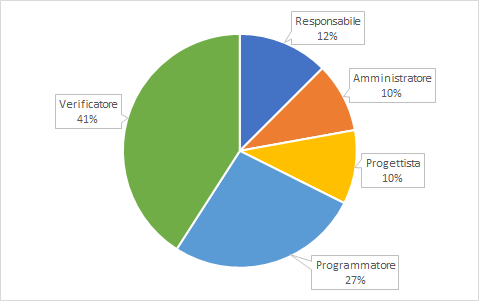
\includegraphics[width=0.7\textwidth]{./res/img/validazioneCollaudo_pe.png}
			\caption{Suddivisione dei ruoli nel periodo di Validazione e collaudo}
		\end{figure}

\subsection{Riepilogo}
	\subsubsection{Ore totali}
		\subsubsubsection{Suddivisione del lavoro}
			Distribuzione totale delle ore per ciascun ruolo comprensive delle ore di investimento e delle ore rendicontate al carico del Committente\ped{\textit{G}}.

			\rowcolors{2}{lightRowColor}{darkRowColor}
			\begin{longtable}{
				>{\centering}p{0.25\textwidth}
				>{\centering}p{0.05\textwidth}
				>{\centering}p{0.05\textwidth}
				>{\centering}p{0.05\textwidth}
				>{\centering}p{0.05\textwidth}
				>{\centering}p{0.05\textwidth}
				>{\centering}p{0.05\textwidth}
				>{\centering\arraybackslash}p{0.15\textwidth} }

				\coloredTableHead
				\textbf{\color{white}Nome} &
				\textbf{\color{white}Rp} &
				\textbf{\color{white}As} &
				\textbf{\color{white}An} &
				\textbf{\color{white}Pt} &
				\textbf{\color{white}Pr} &
				\textbf{\color{white}Vf} &
				\textbf{\color{white}Totale}
				\tabularnewline
				\endhead

				% Contenuto della tabella
				% Nome & Rp & As & An & Pt & Pr & Vf & Totale \\
				\VB & 17 & 24 & 3  & 19 & 34 & 40 & 137 \\
				\LB & 10 & 26 & 10 & 26 & 35 & 30 & 137 \\
				\NF & 5  & 28 & 6  & 37 & 26 & 35 & 137 \\
				\EG & 6  & 13 & 37 & 30 & 26 & 28 & 140 \\
				\FJ & 11 & 17 & 3  & 28 & 31 & 47 & 137 \\
				\MP & 30 & 14 & 2  & 23 & 22 & 46 & 137 \\
				\AS & 6  & 15 & 2  & 21 & 31 & 62 & 137 \\
				\AZ & 7  & 12 & 40 & 14 & 34 & 33 & 140 \\
				\textbf{Ore totali per ruolo} & 92 & 149 & 103 & 198 & 239 & 321 & 1102 \\

				\rowcolor{white}\caption {Suddivisione oraria con il totale delle ore di investimento e rendicontate}	\\

			\end{longtable}

			\newpage
			% Grafico
			Rappresentazione grafica della suddivisione oraria:
			\begin{figure}[h]
				\centering
				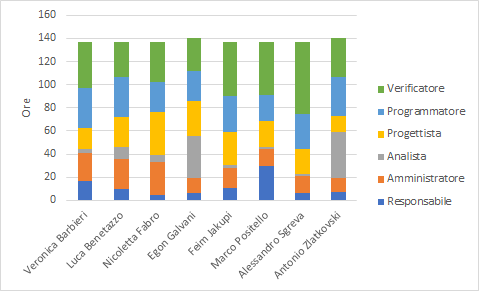
\includegraphics[width=0.7\textwidth]{./res/img/totale_po.png}
				\caption{Suddivisione oraria con il totale delle ore di investimento e rendicontate}
			\end{figure}

		\subsubsubsection{Prospetto econimico}
			Totale delle ore e costo per ciascun ruolo comprensivo delle ore di investimento e delle ore rendicontate a carico del Committente\ped{\textit{G}}:

			\rowcolors{2}{lightRowColor}{darkRowColor}
			\begin{longtable}{
				>{\centering}p{0.25\textwidth}
				>{\centering}p{0.05\textwidth}
				>{\centering\arraybackslash}p{0.15\textwidth} }

				\coloredTableHead
				\textbf{\color{white}Ruolo} &
				\textbf{\color{white}Ore} &
				\textbf{\color{white}Costo in \euro{}}
				\tabularnewline
				\endhead

				% Contenuto della tabella
				% Ruolo & Ore & Costo in \\
				Responsabile    & 92   & 2.760,00 \\
				Amministratore  & 149  & 2.980,00 \\
				Analista        & 103  & 2.575,00 \\
				Progettista     & 198  & 4.356,00 \\
				Programmatore   & 239  & 3.585,00 \\
				Verificatore    & 321  & 4.815,00 \\
				\textbf{Totale} & 1102 & 21.071,00 \\

				\rowcolor{white}\caption {Prospetto dei costi totale delle ore di investimento e rendicontate per ciascun ruolo} \\

			\end{longtable}

			\newpage
			% Grafico
			Rappresentazione grafica della distribuzione dei ruoli:
			\begin{figure}[h]
				\centering
				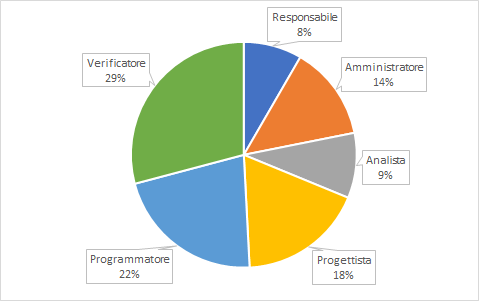
\includegraphics[width=0.7\textwidth]{./res/img/totale_pe.png}
				\caption{Suddivisione dei ruoli per il totale delle ore di investimento e rendicontate }
			\end{figure}

	\subsubsection{Ore rendicontate}
		\subsubsubsection{Suddivisione del lavoro}
			Distribuzione totale delle ore rendicontate per ciascun ruolo.

			\rowcolors{2}{lightRowColor}{darkRowColor}
			\begin{longtable}{
				>{\centering}p{0.25\textwidth}
				>{\centering}p{0.05\textwidth}
				>{\centering}p{0.05\textwidth}
				>{\centering}p{0.05\textwidth}
				>{\centering}p{0.05\textwidth}
				>{\centering}p{0.05\textwidth}
				>{\centering}p{0.05\textwidth}
				>{\centering\arraybackslash}p{0.15\textwidth} }

				\coloredTableHead
				\textbf{\color{white}Nome} &
				\textbf{\color{white}Rp} &
				\textbf{\color{white}As} &
				\textbf{\color{white}An} &
				\textbf{\color{white}Pt} &
				\textbf{\color{white}Pr} &
				\textbf{\color{white}Vf} &
				\textbf{\color{white}Totale}
				\tabularnewline
				\endhead

				% Contenuto della tabella
				% Nome & Rp & As & An & Pt & Pr & Vf & Totale \\
				\VB & 7  & 4  & -  & 19 & 34 & 38 & 102 \\
				\LB & 5  & 6  & 10 & 26 & 35 & 20 & 102 \\
				\NF & 5  & 8  & 6  & 27 & 26 & 30 & 102 \\
				\EG & 6  & 5  & 7  & 30 & 26 & 28 & 102 \\
				\FJ & 11 & 17 & -  & 18 & 31 & 25 & 102 \\
				\MP & 10 & 14 & -  & 23 & 22 & 33 & 102 \\
				\AS & 6  & 10 & -  & 21 & 31 & 34 & 102 \\
				\AZ & 7  & 9  & 10 & 14 & 34 & 28 & 102 \\
				\textbf{Ore totali per ruolo} & 57 & 73 & 33 & 178 & 239 & 236 & 816 \\

				\rowcolor{white}\caption {Suddivisione oraria con il totale delle ore rendicontate} \\

			\end{longtable}

			% Grafico
			Rappresentazione grafica della suddivisione oraria:
			\begin{figure}[h]
				\centering
				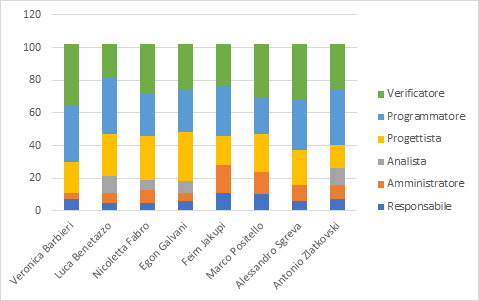
\includegraphics[width=0.7\textwidth]{./res/img/totaleRendicontate_po.png}
				\caption{Suddivisione oraria con il totale delle ore rendicontate}
			\end{figure}

		\newpage
		\subsubsubsection{Prospetto economico}
			Totale delle ore e costo per ciascun ruolo delle ore rendicontate:

			\rowcolors{2}{lightRowColor}{darkRowColor}
			\begin{longtable}{
				>{\centering}p{0.25\textwidth}
				>{\centering}p{0.05\textwidth}
				>{\centering\arraybackslash}p{0.15\textwidth} }

				\coloredTableHead
				\textbf{\color{white}Ruolo} &
				\textbf{\color{white}Ore} &
				\textbf{\color{white}Costo in \euro{}}
				\tabularnewline
				\endhead

				% Contenuto della tabella
				% Ruolo & Ore & Costo in \\
				Responsabile    & 57  & 1.710,00 \\
				Amministratore  & 73  & 1.460,00 \\
				Analista        & 33  & 825,00 \\
				Progettista     & 178 & 3.916,00 \\
				Programmatore   & 239 & 3.585,00 \\
				Verificatore    & 236 & 3.540,00 \\
				\textbf{Totale} & 816 & 15.036,00 \\

				\rowcolor{white}\caption {Prospetto dei costi totale delle ore rendicontate per ciascun ruolo} \\

			\end{longtable}

			\newpage
			% Grafico
			Rappresentazione grafica della distribuzione dei ruoli:
			\begin{figure}[h]
				\centering
				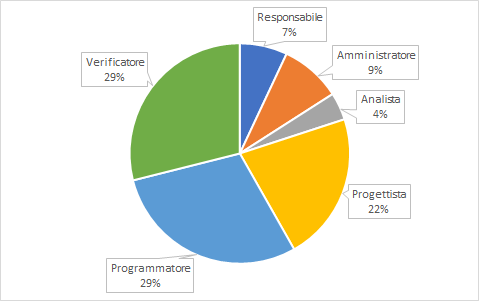
\includegraphics[width=0.7\textwidth]{./res/img/totaleRendicontate_pe.png}
				\caption{Suddivisione dei ruoli per il totale delle ore rendicontate}
			\end{figure}

\subsection{Conclusioni}
		Il costo preventivato totale per il progetto è di \textbf{\euro15.036,00}.

	\pagebreak
	
	\section{Consuntivo di periodo e preventivo a finire}
In questa sezione verranno indicate le spese, totali e per ruolo, sostenute al termine di ciascuna fase.
Il bilancio presentato potrà essere:
\begin{itemize}
	\item \textbf{positivo:} se il totale preventivato è superiore ai valori del consuntivo;
	\item \textbf{pari:} se il totale preventivato è pari ai valori del consuntivo;
	\item \textbf{negativo:} se il totale preventivato è inferiore ai valori del consuntivo.
\end{itemize}
Verrà inoltre presentato un preventivo a finire che terrà conto dei soli periodi rendicontati.

\subsection{Periodo di Analisi}
\subsubsection{Consuntivo di periodo}
\rowcolors{2}{lightRowColor}{darkRowColor}
\begin{longtable}{
		>{\centering}p{0.25\textwidth}
		>{\centering}p{0.08\textwidth}
		>{\centering}p{0.08\textwidth}
		>{\centering}p{0.15\textwidth}
		>{\centering\arraybackslash}p{0.15\textwidth} }
	
	\coloredTableHead
	\textbf{\color{white}Ruolo} &
	\textbf{\color{white}Ore} &
	\textbf{\color{white}Delta ore} &
	\textbf{\color{white}Costo in \euro{}} &
	\textbf{\color{white}Delta costo}
	\tabularnewline
	\endhead
	
	% Contenuto della tabella
	% Ruolo & OreEffettive & DeltaOre & Costo & DeltaCosto \\
	Responsabile    & 28 & -2 &   840,00 & -60 \\
	Amministratore  & 70 & +0 & 1.400,00 & +0,00 \\
	Analista        & 63 & +3 & 1.575,00 & +75,00 \\
	Progettista     & 20 & +0 &   440,00 & +0,00 \\
	Programmatore   & -  & -  & -        & - \\
	Verificatore    & 74 & +4 & 1.110,00 & +60,00 \\
	\textbf{Totale Effettivo} & \multicolumn{2}{c}{\textbf{255}} & \multicolumn{2}{c}{\textbf{5365,00}} \\
	\textbf{Delta} & \multicolumn{2}{c}{\textbf{+4}} & \multicolumn{2}{c}{\textbf{+75,00}} \\
	
	\rowcolor{white}\caption{Consuntivo per il periodo di Analisi}	\\
	
\end{longtable}

\subsubsection{Conclusione}
Come riportato nella tabella del consuntivo per il periodo di Analisi, il preventivo orario per i ruoli di Amministratore e Progettista si è rivelato sufficiente per svolgere il lavoro previsto; si è rivelato  invece necessario dedicare più ore lavorative rispetto a quanto preventivato per i ruoli di Analista e Verificatore, mentre è stato impiegato un monte ore ridotto per il ruolo di Responsabile di Progetto. Di seguito sono riportate le motivazioni:
\begin{itemize}
	\item \textbf{Responsabile di Progetto:} sono state impiegate meno ore rispetto a quelle previste data la minore difficoltà di stesura del \textit{\PdP{} 1.0.0} e di pianificazione del lavoro rispetto a quanto previsto;
	\item \textbf{Analista:} alcuni requisiti hanno presentato delle difficoltà di comprensione, con un conseguente aumento del monte ore necessario per la loro comprensione e stesura all'interno dell'\textit{\AdR{} 1.0.0};
	\item \textbf{Verificatore:} l'aggiornamento delle \textit{\NdP{} 1.0.0} e l'applicazione scorretta di alcune norme causata dall'inesperienza dei membri del gruppo ha portato ad un aumento delle ore spese per questo ruolo.
\end{itemize}

\subsubsection{Preventivo a finire}
Il bilancio finale è negativo. Nonostante ciò, non riteniamo necessario attuare misure di mitigazione o modifiche alla pianificazione dei periodi successivi, in quanto, oltre al fatto che il periodo di Analisi non è rendicontato, siamo riusciti ad individuare le situazioni e le motivazioni che hanno portato a richiedere ore di lavoro aggiuntive rispetto a quelle preventivate. Ciascun componente del gruppo si impegnerà per cercare di evitare che situazioni di questo tipo si possano ripetere nei periodi successivi.


\subsection{Periodo di Consolidamento dei Requisiti}
\subsubsection{Consuntivo di periodo}
\rowcolors{2}{lightRowColor}{darkRowColor}
\begin{longtable}{
		>{\centering}p{0.25\textwidth}
		>{\centering}p{0.08\textwidth}
		>{\centering}p{0.08\textwidth}
		>{\centering}p{0.15\textwidth}
		>{\centering\arraybackslash}p{0.15\textwidth} }
	
	\coloredTableHead
	\textbf{\color{white}Ruolo} &
	\textbf{\color{white}Ore} &
	\textbf{\color{white}Delta ore} &
	\textbf{\color{white}Costo in \euro{}} &
	\textbf{\color{white}Delta costo}
	\tabularnewline
	\endhead
	
	% Contenuto della tabella
	% Ruolo & OreEffettive & DeltaOre & Costo & DeltaCosto \\
	Responsabile    & 5  & +0 & 150,00 & +0,00 \\
	Amministratore  & 6  & +0 & 120,00 & +0,00 \\
	Analista        & 10 & +0 & 250,00 & +0,00 \\
	Progettista     & -  & -  & -       & +0,00 \\
	Programmatore   & -  & -  & -       & +0,00 \\
	Verificatore    & 15 & +0 & 225,00 & +0,00 \\
	\textbf{Totale Effettivo} & \multicolumn{2}{c}{\textbf{36}} & \multicolumn{2}{c}{\textbf{745,00}} \\
	\textbf{Delta} & \multicolumn{2}{c}{\textbf{+0}} & \multicolumn{2}{c}{\textbf{+0,00}} \\
	
	\rowcolor{white}\caption{Consuntivo per il periodo di Consolidamento dei Requisiti}	\\
	
\end{longtable}

\subsubsection{Conclusione}
Il totale delle ore preventivate per il periodo di Consolidamento dei Requisiti si è rivelato corretto per svolgere il lavoro pianificato.
\subsubsection{Preventivo a finire}
Il bilancio finale è pari. Non si rendono quindi necessarie misure di mitigazione o modifiche alla pianificazione dei periodi successivi.

\subsection{Periodo di Progettazione Architetturale}
\subsubsection{Consuntivo di periodo}
\rowcolors{2}{lightRowColor}{darkRowColor}
\begin{longtable}{
		>{\centering}p{0.25\textwidth}
		>{\centering}p{0.08\textwidth}
		>{\centering}p{0.08\textwidth}
		>{\centering}p{0.15\textwidth}
		>{\centering\arraybackslash}p{0.15\textwidth} }
	
	\coloredTableHead
	\textbf{\color{white}Ruolo} &
	\textbf{\color{white}Ore} &
	\textbf{\color{white}Delta ore} &
	\textbf{\color{white}Costo in \euro{}} &
	\textbf{\color{white}Delta costo}
	\tabularnewline
	\endhead
	
	% Contenuto della tabella
	% Ruolo & OreEffettive & DeltaOre & Costo & DeltaCosto \\
	Responsabile    & 12 & +0 &   360,00 & +  0,00 \\
	Amministratore  & 24 & +0 &   480,00 & +  0,00 \\
	Analista        & 35 & +2 &   875,00 & + 50,00 \\
	Progettista     & 67 & -5 & 1.474,00 & -110,00 \\
	Programmatore   & 35 & -4 &   525,00 & - 60,00 \\
	Verificatore    & 68 & +0 & 1.020,00 & +  0,00 \\
	\textbf{Totale Effettivo} & \multicolumn{2}{c}{\textbf{241}} & \multicolumn{2}{c}{\textbf{4.734,00}} \\
	\textbf{Delta} & \multicolumn{2}{c}{\textbf{-7}} & \multicolumn{2}{c}{\textbf{-120,00}} \\
	
	\rowcolor{white}\caption{Consuntivo per il periodo di Progettazione Architetturale}	\\
	
\end{longtable}

\subsubsection{Conclusione}
Come riportato nella tabella del consuntivo per il periodo di Progettazione Architetturale, il preventivo orario per i ruoli di Responsabile, Amministratore e Verificatore si è rivelato sufficiente per svolgere il lavoro pianificato. \\
Si è rivelato necessario dedicare più ore lavorative rispetto a quanto preventivato per il ruolo di Analista, mentre è stato impiegato un monte ore ridotto per i ruoli di Progettista e Programmatore. Di seguito sono riportate le motivazioni:
\begin{itemize}
	\item \textbf{Analista:} la comprensione delle indicazioni ricevute nell'esito della \textit{Revisione dei Requisiti} e la conseguente correzione del documento dell'\textit{AdR{} 2.0.0}, hanno richiesto alcune ore di lavoro in più rispetto a quelle preventivate;
	\item \textbf{Progettista:} le molte ore di studio individuale impiegate nel periodo di Consolidamento dei Requisiti riguardo le tecnologie ritenute potenzialmente utili per lo sviluppo del prodotto\ped{\textit{G}}, hanno permesso di poter impiegare meno ore di quanto pianificato per l'individuazione delle tecnologie e delle librerie adatte allo sviluppo del prodotto\ped{\textit{G}};
	\item \textbf{Programmatore:} grazie alle ore di studio individuali descritte nel punto precedente e all'adeguata scelta delle tecnologie e delle librerie, la codifica del \textit{Proof of Concept} ha richiesto meno ore di lavoro rispetto a quelle preventivate.
\end{itemize}

\subsubsection{Preventivo a finire}
Il bilancio finale è positivo. Ciò è dovuto soprattutto alla scelta iniziale delle tecnologie e delle librerie da utilizzare, che si è rivelata adeguata e ci ha permesso di risparmiare delle ore di lavoro nelle attività di progettazione e di codifica del \textit{Proof of Concept} rispetto a quanto avevamo preventivato. \\
Intendiamo utilizzare l'ammontare risparmiato in questo periodo per assegnare alcune ore supplementari al ruolo dell'Analista nel periodo di Progettazione di Dettaglio e Codifica, in quanto potrebbe essere necessario apportare modifiche al documento dell'\textit{AdR{} 2.0.0}, seguendo eventuali indicazioni ricevute a seguito dell'esito della \textit{Revisione di Progettazione}.

\subsection{Periodo di Progettazione di Dettaglio e Codifica}
Vengono riportati di seguito i consuntivi degli 8 incrementi che costituiscono il periodo considerato. 

\subsubsection{9$^{\circ}$ Incremento}
		\subsubsubsection{Prospetto orario}
		Durante il 9$^{\circ}$ Incremento la distribuzione oraria preventivata dei ruoli di ogni componente del gruppo sarà la seguente:
		\rowcolors{2}{lightRowColor}{darkRowColor}
		\begin{longtable}{
				>{\centering}p{0.25\textwidth}
				>{\centering}p{0.05\textwidth}
				>{\centering}p{0.05\textwidth}
				>{\centering}p{0.05\textwidth}
				>{\centering}p{0.05\textwidth}
				>{\centering}p{0.05\textwidth}
				>{\centering}p{0.05\textwidth}
				>{\centering\arraybackslash}p{0.15\textwidth} }
			
			\coloredTableHead
			\textbf{\color{white}Nome} &
			\textbf{\color{white}Rp} &
			\textbf{\color{white}As} &
			\textbf{\color{white}An} &
			\textbf{\color{white}Pt} &
			\textbf{\color{white}Pr} &
			\textbf{\color{white}Vf} &
			\textbf{\color{white}Totale}
			\tabularnewline
			\endhead
			
			% Contenuto della tabella
			%    Rp & As & An & Pt & Pr & Vf & Totale \\
			\VB & - & 2  & - & - & - & 4 & 6 \\
			\LB & - & -  & - & 4 & - & - & 4 \\
			\NF & - & 4  & - & - & - & - & 4 \\
			\EG & 2 & -  & - & 2 & - & - & 4 \\
			\FJ & - & -  & - & - & - & 4 & 4 \\
			\MP & - & -  & - & 2 & - & 3 & 5 \\
			\AS & - & -  & - & 2 & - & 2 & 4 \\
			\AZ & - & 2  & - & - & - & 2 & 4 \\
			\textbf{Ore totali per ruolo} & 2 & 8 & 0 & 10 & 0 & 15 & 35 \\
			
			\rowcolor{white}\caption {Suddivisione oraria del 9$^{\circ}$ Incremento} \\
			
		\end{longtable}
		
		% Grafico
		\begin{figure}[H]
			\centering
			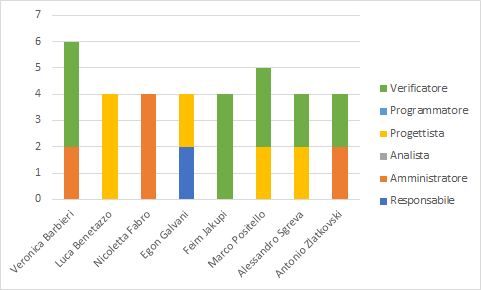
\includegraphics[width=0.7\textwidth]{./res/img/preventivi/inc9_po.png}
			\caption{Suddivisione oraria del 9$^{\circ}$ Incremento}
		\end{figure}
	
		\subsubsubsection{Prospetto economico}
		In base al prospetto orario, quello economico sarà il seguente: 
		\rowcolors{2}{lightRowColor}{darkRowColor}
		\begin{longtable}{
				>{\centering}p{0.25\textwidth}
				>{\centering}p{0.05\textwidth}
				>{\centering\arraybackslash}p{0.15\textwidth} }
			
			\coloredTableHead
			\textbf{\color{white}Ruolo} &
			\textbf{\color{white}Ore} &
			\textbf{\color{white}Costo in \euro{}}
			\tabularnewline
			\endhead
			
			% Contenuto della tabella
			% Ruolo & Ore & Costo \\
			Responsabile    & 2  & 60,00 \\
			Amministratore  & 8  & 160,00 \\
			Analista        & 0  & 0,00 \\
			Progettista     & 10  & 220,00 \\
			Programmatore   & 0  & 0,00 \\
			Verificatore    & 15  & 225,00 \\
			\textbf{Totale} & 35 & 665,00 \\
			
			\rowcolor{white}\caption {Prospetto dei costi per il 9$^{\circ}$ Incremento}	\\
			
		\end{longtable}
		
		% Grafico
		Rappresentazione grafica della distribuzione dei ruoli:
		\begin{figure}[H]
			\centering
			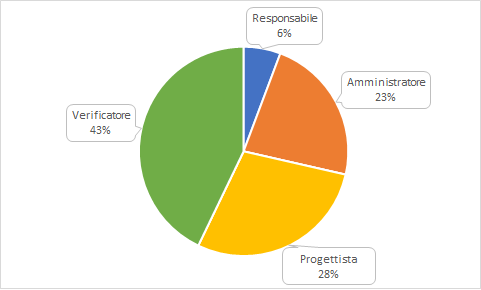
\includegraphics[width=0.7\textwidth]{./res/img/preventivi/inc9_pe.png}
			\caption{Prospetto economico del 9$^{\circ}$ Incremento}
		\end{figure}
\subsubsection{10$^{\circ}$ Incremento}
	
	\subsubsubsection{Consuntivo}
					
		\begin{longtable}{
				>{\centering}p{0.25\textwidth}
				>{\centering}p{0.08\textwidth}
				>{\centering}p{0.08\textwidth}
				>{\centering}p{0.15\textwidth}
				>{\centering\arraybackslash}p{0.15\textwidth} }
			
			\coloredTableHead
			\textbf{\color{white}Ruolo} &
			\textbf{\color{white}Ore} &
			\textbf{\color{white}Delta ore} &
			\textbf{\color{white}Costo in \euro{}} &
			\textbf{\color{white}Delta costo}
			\tabularnewline
			\endhead
			
			% Contenuto della tabella
			% Ruolo & OreEffettive & DeltaOre & Costo & DeltaCosto \\
			Responsabile    & 4 & +0 &   120,00 & +  0,00 \\
			Amministratore  & 4 & +0 &   80,00 & +  0,00 \\
			Analista        & 0 & +0 &   0,00 & + 0,00 \\
			Progettista     & 39 & +4 & 858,00 & + 88,00 \\
			Programmatore   & 23 & -2 &  345,00 & - 30,00 \\
			Verificatore    & 25 & +0 & 375,00 & + 0,00 \\
			\textbf{Totale Effettivo} & \multicolumn{2}{c}{\textbf{95}} & \multicolumn{2}{c}{\textbf{1778,00}} \\
			\textbf{Delta} & \multicolumn{2}{c}{\textbf{+2}} & \multicolumn{2}{c}{\textbf{+58,00}} \\
			
			\rowcolor{white}\caption{Consuntivo per il 10$^{\circ}$ Incremento}	\\
			
		\end{longtable}
		
	\subsubsubsection{Conclusioni}
	In questo periodo il gruppo si è impegnato nella progettazione e scelta dell'architettura da applicare al prodotto\ped{\textit{G}}. Tale procedimento ha richiesto più tempo del previsto, portando alla necessità di un numero di ore superiore a quanto pianificato per il ruolo di Progettista. \\
	L'attività di codifica è stata leggermente meno dispendiosa del previsto, a causa dell'utilizzo del prototipo ottenuto dalla fase precedente. 
	
	\subsubsubsection{Preventivo a finire rispetto al periodo}
	Il bilancio è \textbf{negativo}, con una spesa in eccesso di \textbf{58,00\euro{}}. Non si ritiene necessaria alcuna ripianificazione, poichè la somma non è significativa. 
	Il soddisfacimento degli obiettivi pianificati ha richiesto un quantitativo di ore superiore a quanto previsto, che hanno portato a questo bilancio negativo.
	
	\subsubsubsection{Preventivo a finire complessivo}	
	Date le considerazioni precedenti su costi e obiettivi, il preventivo complessivo resta invariato.
\subsubsection{11$^{\circ}$ Incremento}
	
	\subsubsubsection{Consuntivo}
		\begin{longtable}{
				>{\centering}p{0.25\textwidth}
				>{\centering}p{0.08\textwidth}
				>{\centering}p{0.08\textwidth}
				>{\centering}p{0.15\textwidth}
				>{\centering\arraybackslash}p{0.15\textwidth} }
			
			\coloredTableHead
			\textbf{\color{white}Ruolo} &
			\textbf{\color{white}Ore} &
			\textbf{\color{white}Delta ore} &
			\textbf{\color{white}Costo in \euro{}} &
			\textbf{\color{white}Delta costo}
			\tabularnewline
			\endhead
			
			% Contenuto della tabella
			% Ruolo & OreEffettive & DeltaOre & Costo & DeltaCosto \\
			Responsabile    & 3 & +0 &   90,00 & +  0,00 \\
			Amministratore  & 4 & +0 &   80,00 & +  0,00 \\
			Analista        & 0 & +0 &   0,00 & + 0,00 \\
			Progettista     & 10 & +0 & 220,00 & + 0,00 \\
			Programmatore   & 35 & -7 &   525,00 &  -105,00 \\
			Verificatore    & 15 & +0 & 225,00 & + 0,00 \\
			\textbf{Totale Effettivo} & \multicolumn{2}{c}{\textbf{64}} & \multicolumn{2}{c}{\textbf{1140,00}} \\
			\textbf{Delta} & \multicolumn{2}{c}{\textbf{-10}} & \multicolumn{2}{c}{\textbf{-105,00}} \\
			
			\rowcolor{white}\caption{Consuntivo per l'11$^{\circ}$ Incremento}	\\
			
		\end{longtable}
		
	\subsubsubsection{Conclusioni}
	In questo periodo il gruppo si è impegnato principalmente nell'adattare la struttura del prototipo ottenuto dalla fase precedente alla progettazione identificata nell'Incremento 10. Tale attività ha richiesto un notevole numero di ore di codifica in meno rispetto a quanto previsto, poichè la struttura del prototipo seguiva già in parte quella decisa durante la progettazione. 
	
	\subsubsubsection{Preventivo a finire rispetto al periodo}
	Il bilancio è \textbf{positivo}, con un risparmio di \textbf{105,00\euro{}}.  Tale somma
	andrà a bilanciare il leggero deficit ottenuto nell'Incremento precedente. La differenza
	rispetto ai costi preventivati fino a questo punto sarà quindi poco consistente, perciò non si
	reputa necessaria una ripianificazione delle attività di progetto.
	
	\subsubsubsection{Preventivo a finire complessivo}	
	Date le considerazioni precedenti, il preventivo complessivo resta invariato.
\subsubsection{12$^{\circ}$ Incremento}
		\subsubsubsection{Prospetto orario}
		Durante il 12$^{\circ}$ incremento la distribuzione oraria preventivata dei ruoli di ogni componente del gruppo sarà la seguente:
		\rowcolors{2}{lightRowColor}{darkRowColor}
		\begin{longtable}{
				>{\centering}p{0.25\textwidth}
				>{\centering}p{0.05\textwidth}
				>{\centering}p{0.05\textwidth}
				>{\centering}p{0.05\textwidth}
				>{\centering}p{0.05\textwidth}
				>{\centering}p{0.05\textwidth}
				>{\centering}p{0.05\textwidth}
				>{\centering\arraybackslash}p{0.15\textwidth} }
			
			\coloredTableHead
			\textbf{\color{white}Nome} &
			\textbf{\color{white}Rp} &
			\textbf{\color{white}As} &
			\textbf{\color{white}An} &
			\textbf{\color{white}Pt} &
			\textbf{\color{white}Pr} &
			\textbf{\color{white}Vf} &
			\textbf{\color{white}Totale}
			\tabularnewline
			\endhead
			
			% Contenuto della tabella
			%    Rp & As & An & Pt & Pr & Vf & Totale \\
			\VB & - & -  & - & - & 10 & - & 10 \\
			\LB & - & -  & - & 4 & 10 & - & 14 \\
			\NF & - & -  & - & - & 10 & - & 10 \\
			\EG & - & -  & - & - & 10 & 2 & 12 \\
			\FJ & 2 & -  & - & 4 & - & 1 & 7 \\
			\MP & 1 & -  & - & - & 5 & 2 & 8 \\
			\AS & - & -  & - & 2 & - & 5 & 7 \\
			\AZ & - & 3  & - & - & - & 5 & 8 \\
			\textbf{Ore totali per ruolo} & 3 & 3 & 0 & 10 & 45 & 15 & 76 \\
			
			\rowcolor{white}\caption {Suddivisione oraria del 12$^{\circ}$ incremento} \\
			
		\end{longtable}
		
		% Grafico
		\begin{figure}[H]
			\centering
			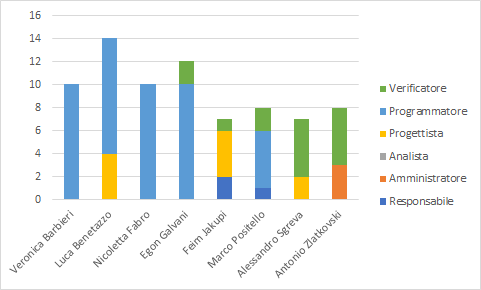
\includegraphics[width=0.7\textwidth]{./res/img/preventivi/inc12_po.png}
			\caption{Suddivisione oraria del 12$^{\circ}$ incremento}
		\end{figure}
	
		\subsubsubsection{Prospetto economico}
		In base al prospetto orario, quello economico sarà il seguente: 
		\rowcolors{2}{lightRowColor}{darkRowColor}
		\begin{longtable}{
				>{\centering}p{0.25\textwidth}
				>{\centering}p{0.05\textwidth}
				>{\centering\arraybackslash}p{0.15\textwidth} }
			
			\coloredTableHead
			\textbf{\color{white}Ruolo} &
			\textbf{\color{white}Ore} &
			\textbf{\color{white}Costo in \euro{}}
			\tabularnewline
			\endhead
			
			% Contenuto della tabella
			% Ruolo & Ore & Costo \\
			Responsabile    & 3  & 90,00 \\
			Amministratore  & 3  & 60,00 \\
			Analista        & 0  & 0,00 \\
			Progettista     & 10  & 220,00 \\
			Programmatore   & 45 & 675,00 \\
			Verificatore    & 15  & 225,00 \\
			\textbf{Totale} & 76 & 1270,00 \\
			
			\rowcolor{white}\caption {Prospetto dei costi per il 12$^{\circ}$ incremento}	\\
			
		\end{longtable}
		
		% Grafico
		Rappresentazione grafica della distribuzione dei ruoli:
		\begin{figure}[H]
			\centering
			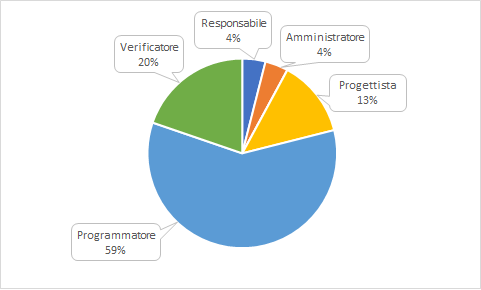
\includegraphics[width=0.7\textwidth]{./res/img/preventivi/inc12_pe.png}
			\caption{Prospetto economico del 12$^{\circ}$ incremento}
		\end{figure}
\subsubsection{13$^{\circ}$ Incremento}
	
	\subsubsubsection{Consuntivo}
		\begin{longtable}{
				>{\centering}p{0.25\textwidth}
				>{\centering}p{0.08\textwidth}
				>{\centering}p{0.08\textwidth}
				>{\centering}p{0.15\textwidth}
				>{\centering\arraybackslash}p{0.15\textwidth} }
			
			\coloredTableHead
			\textbf{\color{white}Ruolo} &
			\textbf{\color{white}Ore} &
			\textbf{\color{white}Delta ore} &
			\textbf{\color{white}Costo in \euro{}} &
			\textbf{\color{white}Delta costo}
			\tabularnewline
			\endhead
			
			% Contenuto della tabella
			% Ruolo & OreEffettive & DeltaOre & Costo & DeltaCosto \\
			Responsabile    & 3 & +0 &   90,00 & +  0,00 \\
			Amministratore  & 3 & +0 &   60,00 & +  0,00 \\
			Analista        & 0 & +0 &   0,00 & + 0,00 \\
			Progettista     & 10 & +0 & 220,00 & + 0,00 \\
			Programmatore   & 27 & -3 &   405,00 &  -45,00 \\
			Verificatore    & 12 & +0 & 180,00 & + 0,00 \\
			\textbf{Totale Effettivo} & \multicolumn{2}{c}{\textbf{55}} & \multicolumn{2}{c}{\textbf{955,00}} \\
			\textbf{Delta} & \multicolumn{2}{c}{\textbf{-3}} & \multicolumn{2}{c}{\textbf{-45,00}} \\
			
			\rowcolor{white}\caption{Consuntivo per il 13$^{\circ}$ Incremento}	\\
			
		\end{longtable}
		
	
	\subsubsubsection{Conclusioni}
	In questo periodo il gruppo si è impegnato principalmente nell'implementare la funzionalità di eliminazione di una funzione dalla piattaforma \textit{Etherless}. L'attività di codifica ha richiesto un numero di ore inferiore a quanto preventivato, in quanto tale funzionalità segue un pattern di comunicazione tra i moduli\ped{\textit{G}} molto simile a quello richiesto da altre funzionalità già implementate. 
	
	\subsubsubsection{Preventivo a finire rispetto al periodo}
	Il bilancio è \textbf{positivo}, con un risparmio di \textbf{45,00\euro{}}. Non si ritiene necessaria alcuna ripianificazione, poichè la somma non è significativa. 
	Gli obiettivi pianificati sono stati raggiunti nei tempi stabiliti, consentendo l'avanzamento delle attività senza ritardi.
	
	\subsubsubsection{Preventivo a finire complessivo}	
	Date le considerazioni precedenti, il preventivo complessivo resta invariato.
\subsubsection{14$^{\circ}$ Incremento}
		\subsubsubsection{Prospetto orario}
		Durante il quattordicesimo incremento la distribuzione oraria preventivata dei ruoli di ogni componente del gruppo sarà la seguente:
		\rowcolors{2}{lightRowColor}{darkRowColor}
		\begin{longtable}{
				>{\centering}p{0.25\textwidth}
				>{\centering}p{0.05\textwidth}
				>{\centering}p{0.05\textwidth}
				>{\centering}p{0.05\textwidth}
				>{\centering}p{0.05\textwidth}
				>{\centering}p{0.05\textwidth}
				>{\centering}p{0.05\textwidth}
				>{\centering\arraybackslash}p{0.15\textwidth} }
			
			\coloredTableHead
			\textbf{\color{white}Nome} &
			\textbf{\color{white}Rp} &
			\textbf{\color{white}As} &
			\textbf{\color{white}An} &
			\textbf{\color{white}Pt} &
			\textbf{\color{white}Pr} &
			\textbf{\color{white}Vf} &
			\textbf{\color{white}Totale}
			\tabularnewline
			\endhead
			
			% Contenuto della tabella
			%    Rp & As & An & Pt & Pr & Vf & Totale \\
			\VB & 3 & -  & - & 3 & - & - & 6 \\
			\LB & - & -  & - & 3 & - & - & 3 \\
			\NF & - & -  & - & 2 & 1 & - & 3 \\
			\EG & - & -  & - & - & 2 & 6 & 8 \\
			\FJ & - & 1  & - & - & 3 & - & 4 \\
			\MP & - & 3  & - & - & 2 & - & 5 \\
			\AS & - & -  & - & - & 3 & 4 & 7 \\
			\AZ & - & -  & - & - & 5 & - & 5 \\
			\textbf{Ore totali per ruolo} & 3 & 4 & 0 & 8 & 16 & 10 & 41 \\
			
			\rowcolor{white}\caption {Suddivisione oraria del quattordicesimo incremento} \\
			
		\end{longtable}
		
		% Grafico
		\begin{figure}[h]
			\centering
			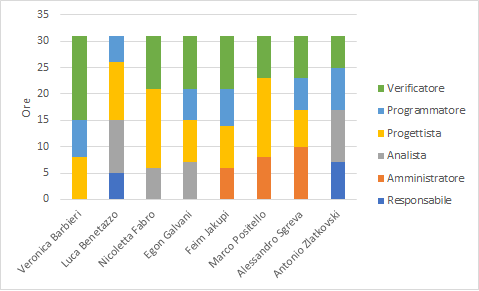
\includegraphics[width=0.7\textwidth]{./res/img/progettazioneArchitetturale_po.png}
			\caption{Suddivisione oraria del quattordicesimo incremento}
		\end{figure}
	
		\subsubsubsection{Prospetto economico}
		In base al prospetto orario, quello economico sarà il seguente: 
		\rowcolors{2}{lightRowColor}{darkRowColor}
		\begin{longtable}{
				>{\centering}p{0.25\textwidth}
				>{\centering}p{0.05\textwidth}
				>{\centering\arraybackslash}p{0.15\textwidth} }
			
			\coloredTableHead
			\textbf{\color{white}Ruolo} &
			\textbf{\color{white}Ore} &
			\textbf{\color{white}Costo in \euro{}}
			\tabularnewline
			\endhead
			
			% Contenuto della tabella
			% Ruolo & Ore & Costo \\
			Responsabile    & 3  & 90,00 \\
			Amministratore  & 4  & 80,00 \\
			Analista        & 0  & 0,00 \\
			Progettista     & 8  & 176,00 \\
			Programmatore   & 16  & 240,00 \\
			Verificatore    & 10  & 150,00 \\
			\textbf{Totale} & 41 & 736,00 \\
			
			\rowcolor{white}\caption {Prospetto dei costi per il quattordicesimo incremento}	\\
			
		\end{longtable}
		
		% Grafico
		Rappresentazione grafica della distribuzione dei ruoli:
		\begin{figure}[h]
			\centering
			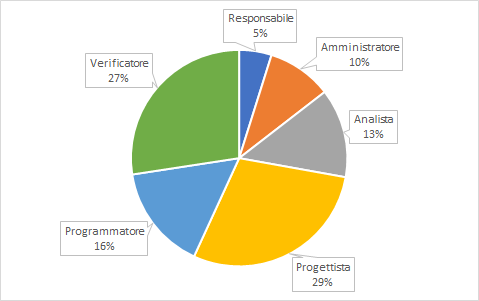
\includegraphics[width=0.7\textwidth]{./res/img/progettazioneArchitetturale_pe.png}
			\caption{Prospetto economico del quattordicesimo incremento}
		\end{figure}
\subsubsection{15$^{\circ}$ Incremento}
		\subsubsubsection{Prospetto orario}
		Durante il quindicesimo incremento la distribuzione oraria preventivata dei ruoli di ogni componente del gruppo sarà la seguente:
		\rowcolors{2}{lightRowColor}{darkRowColor}
		\begin{longtable}{
				>{\centering}p{0.25\textwidth}
				>{\centering}p{0.05\textwidth}
				>{\centering}p{0.05\textwidth}
				>{\centering}p{0.05\textwidth}
				>{\centering}p{0.05\textwidth}
				>{\centering}p{0.05\textwidth}
				>{\centering}p{0.05\textwidth}
				>{\centering\arraybackslash}p{0.15\textwidth} }
			
			\coloredTableHead
			\textbf{\color{white}Nome} &
			\textbf{\color{white}Rp} &
			\textbf{\color{white}As} &
			\textbf{\color{white}An} &
			\textbf{\color{white}Pt} &
			\textbf{\color{white}Pr} &
			\textbf{\color{white}Vf} &
			\textbf{\color{white}Totale}
			\tabularnewline
			\endhead
			
			% Contenuto della tabella
			%    Rp & As & An & Pt & Pr & Vf & Totale \\
			\VB & 1 & -  & - & - & - & - & 1 \\
			\LB & - & -  & - & - & - & - & 0 \\
			\NF & - & -  & - & - & - & - & 0 \\
			\EG & - & -  & - & - & - & - & 0 \\
			\FJ & - & 4  & - & - & - & - & 4 \\
			\MP & 2 & -  & - & - & - & - & 2 \\
			\AS & - & -  & - & - & 1 & 2 & 3 \\
			\AZ & - & -  & - & 2 & - & - & 2 \\
			\textbf{Ore totali per ruolo} & 3 & 4 & 0 & 2 & 1 & 2 & 12 \\
			
			\rowcolor{white}\caption {Suddivisione oraria del quindicesimo incremento} \\
			
		\end{longtable}
		
		% Grafico
		\begin{figure}[H]
			\centering
			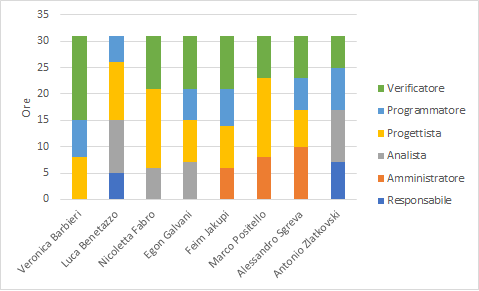
\includegraphics[width=0.7\textwidth]{./res/img/progettazioneArchitetturale_po.png}
			\caption{Suddivisione oraria del quindicesimo incremento}
		\end{figure}
	
		\subsubsubsection{Prospetto economico}
		In base al prospetto orario, quello economico sarà il seguente: 
		\rowcolors{2}{lightRowColor}{darkRowColor}
		\begin{longtable}{
				>{\centering}p{0.25\textwidth}
				>{\centering}p{0.05\textwidth}
				>{\centering\arraybackslash}p{0.15\textwidth} }
			
			\coloredTableHead
			\textbf{\color{white}Ruolo} &
			\textbf{\color{white}Ore} &
			\textbf{\color{white}Costo in \euro{}}
			\tabularnewline
			\endhead
			
			% Contenuto della tabella
			% Ruolo & Ore & Costo \\
			Responsabile    & 3  & 90,00 \\
			Amministratore  & 4  & 80,00 \\
			Analista        & 0  & 0,00 \\
			Progettista     & 2  & 44,00 \\
			Programmatore   & 1  & 15,00 \\
			Verificatore    & 2  & 30,00 \\
			\textbf{Totale} & 12 & 259,00 \\
			
			\rowcolor{white}\caption {Prospetto dei costi per il quindicesimo incremento}	\\
			
		\end{longtable}
		
		% Grafico
		Rappresentazione grafica della distribuzione dei ruoli:
		\begin{figure}[H]
			\centering
			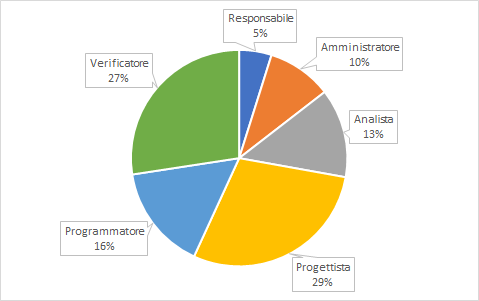
\includegraphics[width=0.7\textwidth]{./res/img/progettazioneArchitetturale_pe.png}
			\caption{Prospetto economico del quindicesimo incremento}
		\end{figure}
\subsubsection{16$^{\circ}$ Incremento}
		\subsubsubsection{Prospetto orario}
		Durante il 16$^{\circ}$ incremento la distribuzione oraria preventivata dei ruoli di ogni componente del gruppo sarà la seguente:
		\rowcolors{2}{lightRowColor}{darkRowColor}
		\begin{longtable}{
				>{\centering}p{0.25\textwidth}
				>{\centering}p{0.05\textwidth}
				>{\centering}p{0.05\textwidth}
				>{\centering}p{0.05\textwidth}
				>{\centering}p{0.05\textwidth}
				>{\centering}p{0.05\textwidth}
				>{\centering}p{0.05\textwidth}
				>{\centering\arraybackslash}p{0.15\textwidth} }
			
			\coloredTableHead
			\textbf{\color{white}Nome} &
			\textbf{\color{white}Rp} &
			\textbf{\color{white}As} &
			\textbf{\color{white}An} &
			\textbf{\color{white}Pt} &
			\textbf{\color{white}Pr} &
			\textbf{\color{white}Vf} &
			\textbf{\color{white}Totale}
			\tabularnewline
			\endhead
			
			% Contenuto della tabella
			%    Rp & As & An & Pt & Pr & Vf & Totale \\
			\VB & - & -  & - & - & - & - & 0 \\
			\LB & - & -  & - & - & - & - & 0 \\
			\NF & - & -  & - & - & - & - & 0 \\
			\EG & - & -  & - & - & - & - & 0 \\
			\FJ & - & -  & - & - & - & - & 0 \\
			\MP & 2 & -  & - & - & - & - & 2 \\
			\AS & - & -  & - & - & 1 & 2 & 3 \\
			\AZ & - & 2  & - & 3 & - & - & 5 \\
			\textbf{Ore totali per ruolo} & 2 & 2 & 0 & 3 & 1 & 2 & 10 \\
			
			\rowcolor{white}\caption {Suddivisione oraria del 16$^{\circ}$ incremento} \\
			
		\end{longtable}
		
		% Grafico
		\begin{figure}[H]
			\centering
			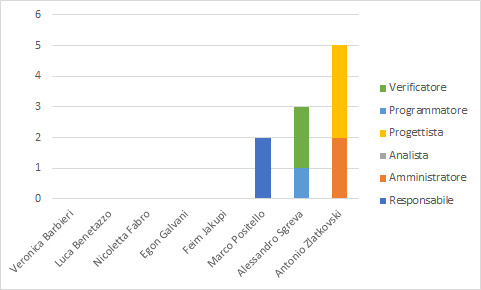
\includegraphics[width=0.7\textwidth]{./res/img/preventivi/inc16_po.png}
			\caption{Suddivisione oraria del 16$^{\circ}$ incremento}
		\end{figure}
	
		\subsubsubsection{Prospetto economico}
		In base al prospetto orario, quello economico sarà il seguente: 
		\rowcolors{2}{lightRowColor}{darkRowColor}
		\begin{longtable}{
				>{\centering}p{0.25\textwidth}
				>{\centering}p{0.05\textwidth}
				>{\centering\arraybackslash}p{0.15\textwidth} }
			
			\coloredTableHead
			\textbf{\color{white}Ruolo} &
			\textbf{\color{white}Ore} &
			\textbf{\color{white}Costo in \euro{}}
			\tabularnewline
			\endhead
			
			% Contenuto della tabella
			% Ruolo & Ore & Costo \\
			Responsabile    & 2  & 60,00 \\
			Amministratore  & 2  & 40,00 \\
			Analista        & 0  & 0,00 \\
			Progettista     & 3  & 66,00 \\
			Programmatore   & 1  & 15,00 \\
			Verificatore    & 2  & 30,00 \\
			\textbf{Totale} & 10 & 211,00 \\
			
			\rowcolor{white}\caption {Prospetto dei costi per il 16$^{\circ}$ incremento}	\\
			
		\end{longtable}
		
		% Grafico
		Rappresentazione grafica della distribuzione dei ruoli:
		\begin{figure}[H]
			\centering
			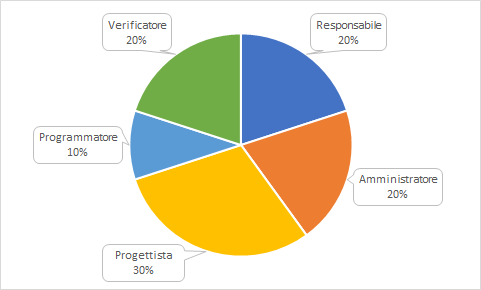
\includegraphics[width=0.7\textwidth]{./res/img/preventivi/inc16_pe.png}
			\caption{Prospetto economico del 16$^{\circ}$ incremento}
		\end{figure}
\subsubsection{Periodo complessivo}

	\subsubsubsection{Consuntivo}
		\begin{longtable}{
			>{\centering}p{0.25\textwidth}
			>{\centering}p{0.08\textwidth}
			>{\centering}p{0.08\textwidth}
			>{\centering}p{0.15\textwidth}
			>{\centering\arraybackslash}p{0.15\textwidth} }
		
		\coloredTableHead
		\textbf{\color{white}Ruolo} &
		\textbf{\color{white}Ore} &
		\textbf{\color{white}Delta ore} &
		\textbf{\color{white}Costo in \euro{}} &
		\textbf{\color{white}Delta costo}
		\tabularnewline
		\endhead
		
		% Contenuto della tabella
		% Ruolo & OreEffettive & DeltaOre & Costo & DeltaCosto \\
		Responsabile    & 23 & +0 &   690,00 & +  0,00 \\
		Amministratore  & 26 & -6 &   520,00 & -  120,00 \\
		Analista        & 3 & +3 &   75,00 & + 75,00 \\
		Progettista     & 94 & +6 & 2068,00 & + 132,00 \\
		Programmatore   & 145 & -8 &   2175,00 &  -120,00 \\
		Verificatore    & 98 & +2 & 1470,00 & + 30,00 \\
		\textbf{Totale Effettivo} & \multicolumn{2}{c}{\textbf{389}} & \multicolumn{2}{c}{\textbf{6998,00}} \\
		\textbf{Delta} & \multicolumn{2}{c}{\textbf{-3}} & \multicolumn{2}{c}{\textbf{-3,00}} \\
		
		\rowcolor{white}\caption{Consuntivo per il periodo di Progettazione di Dettaglio e Codifica}	\\
		
	\end{longtable}
	
	\subsubsubsection{Conclusioni}
	Il bilancio finale è \textbf{positivo}, con un risparmio di \textbf{3,00\euro}. \\ Come riportato nella tabella del consuntivo per il periodo di Progettazione di Dettaglio e Codifica, il numero di ore preventivate per il ruolo di Responsabile si è dimostrato adeguato. \\ Segue un'analisi delle motivazioni per cui gli altri ruoli hanno necessitato di un numero di ore differente da quanto previsto: 
	\begin{itemize}
		\item \textbf{Amministratore}: il numero limitato di modifiche da apportare alle \NdP hanno portato ad un risparmio di ore;
		\item \textbf{Analista}: al contrario di quanto previsto, è stato necessario apportare ulteriori modifiche all'\AdR, questo ha portato alla necessità di alcune ore di lavoro non preventivate;
		\item \textbf{Progettista}: la scarsa conoscenza dei design pattern e l'esito della Product Baseline hanno portato ad un incremento considerevole delle ore di lavoro richieste da tale ruolo;
		\item \textbf{Programmatore}: il riutilizzo del prototipo creato per la \textit{Technology Baseline} e la ripetizione di pattern di comunicazione tra i vari moduli hanno permesso di risparmiare alcune ore di lavoro;
		\item \textbf{Verificatore}: sono state necessarie alcune ore di lavoro non preventivate per verificare tutte le modifiche apportate alla documentazione;
	\end{itemize}
	
	\subsubsubsection{Preventivo a finire}	
	Date le considerazioni precedenti il preventivo complessivo resta invariato. In particolare il risparmio ottenuto in questo periodo risulta essere alquanto ridotto, e per questo non porta ad alcuna ripianificazione. 
	
	

\subsection{Periodo di Validazione e Collaudo}
Vengono riportati di seguito i consuntivi dei 7 incrementi che costituiscono il periodo considerato. 

\subsubsection{17$^{\circ}$ Incremento}
		\subsubsubsection{Prospetto orario}
		Durante il 17$^{\circ}$ incremento la distribuzione oraria preventivata dei ruoli di ogni componente del gruppo sarà la seguente:
		\rowcolors{2}{lightRowColor}{darkRowColor}
		\begin{longtable}{
				>{\centering}p{0.25\textwidth}
				>{\centering}p{0.05\textwidth}
				>{\centering}p{0.05\textwidth}
				>{\centering}p{0.05\textwidth}
				>{\centering}p{0.05\textwidth}
				>{\centering}p{0.05\textwidth}
				>{\centering}p{0.05\textwidth}
				>{\centering\arraybackslash}p{0.15\textwidth} }
			
			\coloredTableHead
			\textbf{\color{white}Nome} &
			\textbf{\color{white}Rp} &
			\textbf{\color{white}As} &
			\textbf{\color{white}An} &
			\textbf{\color{white}Pt} &
			\textbf{\color{white}Pr} &
			\textbf{\color{white}Vf} &
			\textbf{\color{white}Totale}
			\tabularnewline
			\endhead
			
			% Contenuto della tabella
			%    Rp & As & An & Pt & Pr & Vf & Totale \\
			\VB & - & -  & - & 3 & - & 2 & 5 \\
			\LB & - & 3  & - & - & - & - & 3 \\
			\NF & 3 & -  & - & - & - & - & 3 \\
			\EG & - & 3  & - & - & - & 2 & 5 \\
			\FJ & 4 & -  & - & - & - & - & 4 \\
			\MP & - & -  & - & - & 3 & - & 3 \\
			\AS & - & -  & - & - & 2 & - & 2 \\
			\AZ & - & -  & - & - & - & 5 & 5 \\
			\textbf{Ore totali per ruolo} & 7 & 6 & 0 & 3 & 5 & 9 & 30 \\
			
			\rowcolor{white}\caption {Suddivisione oraria del 17$^{\circ}$ incremento} \\
			
		\end{longtable}
		
		% Grafico
		\begin{figure}[H]
			\centering
			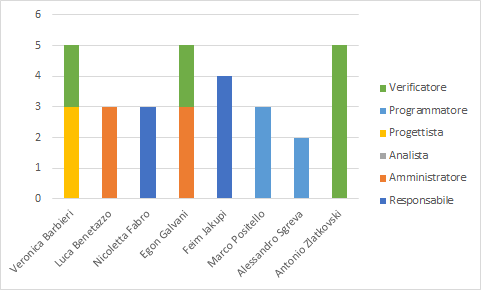
\includegraphics[width=0.7\textwidth]{./res/img/preventivi/inc17_po.png}
			\caption{Suddivisione oraria del 17$^{\circ}$ incremento}
		\end{figure}
	
		\subsubsubsection{Prospetto economico}
		In base al prospetto orario, quello economico sarà il seguente: 
		\rowcolors{2}{lightRowColor}{darkRowColor}
		\begin{longtable}{
				>{\centering}p{0.25\textwidth}
				>{\centering}p{0.05\textwidth}
				>{\centering\arraybackslash}p{0.15\textwidth} }
			
			\coloredTableHead
			\textbf{\color{white}Ruolo} &
			\textbf{\color{white}Ore} &
			\textbf{\color{white}Costo in \euro{}}
			\tabularnewline
			\endhead
			
			% Contenuto della tabella
			% Ruolo & Ore & Costo \\
			Responsabile    & 7  & 210,00 \\
			Amministratore  & 6  & 120,00 \\
			Analista        & 0  & 0,00 \\
			Progettista     & 3  & 66,00 \\
			Programmatore   & 5  & 75,00 \\
			Verificatore    & 9  & 135,00 \\
			\textbf{Totale} & 30 & 606,00 \\
			
			\rowcolor{white}\caption {Prospetto dei costi per il 17$^{\circ}$ incremento}	\\
			
		\end{longtable}
		
		% Grafico
		Rappresentazione grafica della distribuzione dei ruoli:
		\begin{figure}[H]
			\centering
			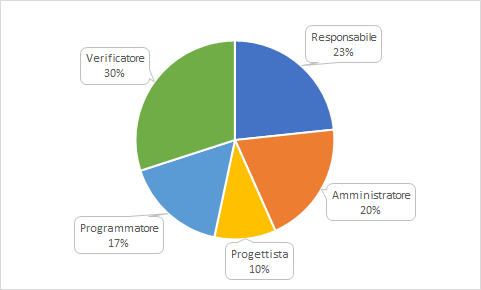
\includegraphics[width=0.7\textwidth]{./res/img/preventivi/inc17_pe.png}
			\caption{Prospetto economico del 17$^{\circ}$ incremento}
		\end{figure}
\subsubsection{18$^{\circ}$ Incremento}

	\subsubsubsection{Consuntivo}
		\begin{longtable}{
				>{\centering}p{0.25\textwidth}
				>{\centering}p{0.08\textwidth}
				>{\centering}p{0.08\textwidth}
				>{\centering}p{0.15\textwidth}
				>{\centering\arraybackslash}p{0.15\textwidth} }

			\coloredTableHead
			\textbf{\color{white}Ruolo} &
			\textbf{\color{white}Ore} &
			\textbf{\color{white}Delta ore} &
			\textbf{\color{white}Costo in \euro{}} &
			\textbf{\color{white}Delta costo}
			\tabularnewline
			\endhead

			% Contenuto della tabella
			% Ruolo & OreEffettive & DeltaOre & Costo & DeltaCosto \\
      Responsabile    & 1  & +0 & 30,00  & +  0,00 \\
      Amministratore  & 1  & +0 & 20,00  & +  0,00 \\
      Analista        & 0  & +0 & 0,00   & +  0,00 \\
      Progettista     & 3  & +0 & 66,00  & +  0,00 \\
      Programmatore   & 10 & +0 & 150,00 & +  0,00 \\
      Verificatore    & 15 & +0 & 225,00 & +  0,00 \\
			\textbf{Totale Effettivo} & \multicolumn{2}{c}{\textbf{30}} & \multicolumn{2}{c}{\textbf{491,00}} \\
			\textbf{Delta} & \multicolumn{2}{c}{\textbf{0}} & \multicolumn{2}{c}{\textbf{+0,00}} \\

			\rowcolor{white}\caption{Consuntivo per il 18$^{\circ}$ Incremento}	\\

		\end{longtable}

	\subsubsubsection{Conclusioni}
	In questo periodo ci siamo dedicati all'implementazione della funzionalità di \texttt{init} (visualizzazione informazioni utili per iniziare ad utilizzare l'applicativo), \texttt{whoami} (visualizzazione dell'indirizzo dell'utente attualmente autenticato nel sistema) e \texttt{search} (ricerca di una funzione). Queste funzionalità richiedono solamente modifiche al modulo \textit{Etherless-cli}, e sono state rispettate il monte ore e le scadenze previste.

	\subsubsubsection{Preventivo a finire rispetto al periodo}
	La pianificazione in questo incremento è stata rispettata e il bilancio risulta essere \textbf{pari}.

	\subsubsubsection{Preventivo a finire complessivo}
	Date le considerazioni precedenti, il preventivo complessivo resta invariato.

\subsubsection{19$^{\circ}$ Incremento}
		
	\subsubsubsection{Consuntivo}
		\begin{longtable}{
				>{\centering}p{0.25\textwidth}
				>{\centering}p{0.08\textwidth}
				>{\centering}p{0.08\textwidth}
				>{\centering}p{0.15\textwidth}
				>{\centering\arraybackslash}p{0.15\textwidth} }
			
			\coloredTableHead
			\textbf{\color{white}Ruolo} &
			\textbf{\color{white}Ore} &
			\textbf{\color{white}Delta ore} &
			\textbf{\color{white}Costo in \euro{}} &
			\textbf{\color{white}Delta costo}
			\tabularnewline
			\endhead
			
			% Contenuto della tabella
			% Ruolo & OreEffettive & DeltaOre & Costo & DeltaCosto \\
			Responsabile    & 1 & +0 &   30,00 & +  0,00 \\
			Amministratore  & 1 & +0 &   20,00 & +  0,00 \\
			Analista        & 0 & +0 &   0,00 & + 0,00 \\
			Progettista     & 2 & +0 & 44,00 & + 0,00 \\
			Programmatore   & 8 & +0 &   120,00 &  +0,00 \\
			Verificatore    & 5 & +0 & 75,00 & + 0,00 \\
			\textbf{Totale Effettivo} & \multicolumn{2}{c}{\textbf{17}} & \multicolumn{2}{c}{\textbf{289,00}} \\
			\textbf{Delta} & \multicolumn{2}{c}{\textbf{0}} & \multicolumn{2}{c}{\textbf{+0,00}} \\
			
			\rowcolor{white}\caption{Consuntivo per il 19$^{\circ}$ Incremento}	\\
			
		\end{longtable}
		
	
	\subsubsubsection{Conclusioni}
	In questo periodo il gruppo si è dedicato principalmente all'implementazione della funzionalità di visualizzazione della cronologia di esecuzione dell'utente. Poichè tale funzionalità richiede delle modifiche unicamente al modulo\ped{\textit{G}} \textit{Etherless-cli} il gruppo è riuscito a rispettare la pianificazione. 
		
	\subsubsubsection{Preventivo a finire rispetto al periodo}
	La pianificazione in questo incremento è stata rispettata e il bilancio risulta essere \textbf{pari}. 
		
	\subsubsubsection{Preventivo a finire complessivo}	
	Date le considerazioni precedenti, il preventivo complessivo resta invariato.
\subsubsection{20$^{\circ}$ Incremento}
		
	\subsubsubsection{Consuntivo}
		\begin{longtable}{
				>{\centering}p{0.25\textwidth}
				>{\centering}p{0.08\textwidth}
				>{\centering}p{0.08\textwidth}
				>{\centering}p{0.15\textwidth}
				>{\centering\arraybackslash}p{0.15\textwidth} }
			
			\coloredTableHead
			\textbf{\color{white}Ruolo} &
			\textbf{\color{white}Ore} &
			\textbf{\color{white}Delta ore} &
			\textbf{\color{white}Costo in \euro{}} &
			\textbf{\color{white}Delta costo}
			\tabularnewline
			\endhead
			
			% Contenuto della tabella
			% Ruolo & OreEffettive & DeltaOre & Costo & DeltaCosto \\
			Responsabile    & 1 & +0 &   30,00 & +  0,00 \\
			Amministratore  & 1 & +0 &   20,00 & +  0,00 \\
			Analista        & 0 & +0 &   0,00 & + 0,00 \\
			Progettista     & 2 & +0 &  44,00 & + 0,00 \\
			Programmatore   & 9 & +4 &   105,00 &  +30,00 \\
			Verificatore    & 5 & +0 & 75,00 & + 0,00 \\
			\textbf{Totale Effettivo} & \multicolumn{2}{c}{\textbf{18}} & \multicolumn{2}{c}{\textbf{274,00}} \\
			\textbf{Delta} & \multicolumn{2}{c}{\textbf{+4}} & \multicolumn{2}{c}{\textbf{+30,00}} \\
			
			\rowcolor{white}\caption{Consuntivo per il 20$^{\circ}$ Incremento}	\\
			
		\end{longtable}
		
	
	\subsubsubsection{Conclusioni}
	In questo periodo il gruppo si è dedicato principalmente all'implementazione della funzionalità di modifica di una funzione. Pur seguendo un pattern di comunicazione tra moduli già utilizzato dal gruppo, l'implementazione della funzionalità ha richiesto più tempo di quanto preventivato. 
	
	\subsubsubsection{Preventivo a finire rispetto al periodo}
	Sono state utilizzare 4 ore di lavoro non preventivate da parte dei Programmatori; questo ha portato ad un bilancio \textbf{negativo}, con una spesa in eccesso di \textbf{30,00\euro}. 
		
	\subsubsubsection{Preventivo a finire complessivo}	
	Non essendo tale spesa eccessiva e avendo ottenuto un risparmio nei periodi precedenti, il preventivo complessivo resta invariato.
\subsubsection{21$^{\circ}$ Incremento}
		\subsubsubsection{Prospetto orario}
		Durante il 21$^{\circ}$ incremento la distribuzione oraria preventivata dei ruoli di ogni componente del gruppo sarà la seguente:
		\rowcolors{2}{lightRowColor}{darkRowColor}
		\begin{longtable}{
				>{\centering}p{0.25\textwidth}
				>{\centering}p{0.05\textwidth}
				>{\centering}p{0.05\textwidth}
				>{\centering}p{0.05\textwidth}
				>{\centering}p{0.05\textwidth}
				>{\centering}p{0.05\textwidth}
				>{\centering}p{0.05\textwidth}
				>{\centering\arraybackslash}p{0.15\textwidth} }
			
			\coloredTableHead
			\textbf{\color{white}Nome} &
			\textbf{\color{white}Rp} &
			\textbf{\color{white}As} &
			\textbf{\color{white}An} &
			\textbf{\color{white}Pt} &
			\textbf{\color{white}Pr} &
			\textbf{\color{white}Vf} &
			\textbf{\color{white}Totale}
			\tabularnewline
			\endhead
			
			% Contenuto della tabella
			%    Rp & As & An & Pt & Pr & Vf & Totale \\
			\VB & - & -  & - & - & 2 & 5 & 7 \\
			\LB & - & -  & - & - & 4 & - & 4 \\
			\NF & - & -  & - & - & 3 & 5 & 8 \\
			\EG & - & -  & - & 2 & - & 1 & 3 \\
			\FJ & - & 3  & - & - & 2 & - & 5 \\
			\MP & 3 & -  & - & - & 1 & 5 & 9 \\
			\AS & - & -  & - & - & 1 & 6 & 7 \\
			\AZ & - & -  & - & 2 & 3 & - & 5 \\
			\textbf{Ore totali per ruolo} & 3 & 3 & 0 & 4 & 16 & 22 & 48 \\
			
			\rowcolor{white}\caption {Suddivisione oraria del 21$^{\circ}$ incremento} \\
			
		\end{longtable}
		
		% Grafico
		\begin{figure}[H]
			\centering
			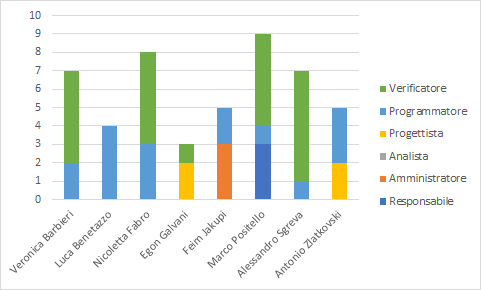
\includegraphics[width=0.7\textwidth]{./res/img/preventivi/inc21_po.png}
			\caption{Suddivisione oraria del 21$^{\circ}$ incremento}
		\end{figure}
	
		\subsubsubsection{Prospetto economico}
		In base al prospetto orario, quello economico sarà il seguente: 
		\rowcolors{2}{lightRowColor}{darkRowColor}
		\begin{longtable}{
				>{\centering}p{0.25\textwidth}
				>{\centering}p{0.05\textwidth}
				>{\centering\arraybackslash}p{0.15\textwidth} }
			
			\coloredTableHead
			\textbf{\color{white}Ruolo} &
			\textbf{\color{white}Ore} &
			\textbf{\color{white}Costo in \euro{}}
			\tabularnewline
			\endhead
			
			% Contenuto della tabella
			% Ruolo & Ore & Costo \\
			Responsabile    & 3  & 90,00 \\
			Amministratore  & 3  & 60,00 \\
			Analista        & 0  & 0,00 \\
			Progettista     & 4  & 88,00 \\
			Programmatore   & 16  & 240,00 \\
			Verificatore    & 22  & 330,00 \\
			\textbf{Totale} & 48 & 808,00 \\
			
			\rowcolor{white}\caption {Prospetto dei costi per il 21$^{\circ}$ incremento}	\\
			
		\end{longtable}
		
		% Grafico
		Rappresentazione grafica della distribuzione dei ruoli:
		\begin{figure}[H]
			\centering
			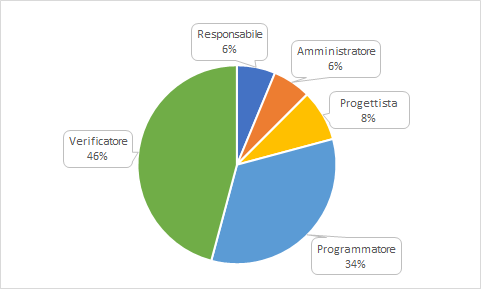
\includegraphics[width=0.7\textwidth]{./res/img/preventivi/inc21_pe.png}
			\caption{Prospetto economico del 21$^{\circ}$ incremento}
		\end{figure}
\subsubsection{22$^{\circ}$ Incremento}
		\subsubsubsection{Prospetto orario}
		Durante il 22$^{\circ}$ Incremento la distribuzione oraria preventivata dei ruoli di ogni componente del gruppo sarà la seguente:
		\rowcolors{2}{lightRowColor}{darkRowColor}
		\begin{longtable}{
				>{\centering}p{0.25\textwidth}
				>{\centering}p{0.05\textwidth}
				>{\centering}p{0.05\textwidth}
				>{\centering}p{0.05\textwidth}
				>{\centering}p{0.05\textwidth}
				>{\centering}p{0.05\textwidth}
				>{\centering}p{0.05\textwidth}
				>{\centering\arraybackslash}p{0.15\textwidth} }
			
			\coloredTableHead
			\textbf{\color{white}Nome} &
			\textbf{\color{white}Rp} &
			\textbf{\color{white}As} &
			\textbf{\color{white}An} &
			\textbf{\color{white}Pt} &
			\textbf{\color{white}Pr} &
			\textbf{\color{white}Vf} &
			\textbf{\color{white}Totale}
			\tabularnewline
			\endhead
			
			% Contenuto della tabella
			%    Rp & As & An & Pt & Pr & Vf & Totale \\
			\VB & - & -  & - & - & - & 2 & 2 \\
			\LB & - & -  & - & - & 2 & 3 & 5 \\
			\NF & - & -  & - & - & - & 5 & 5 \\
			\EG & - & 2  & - & 1 & - & 3 & 6 \\
			\FJ & - & 2  & - & - & - & - & 2 \\
			\MP & 2 & -  & - & - & - & - & 2 \\
			\AS & 5 & -  & - & - & - & - & 5 \\
			\AZ & - & -  & - & 2 & - & 1 & 3 \\
			\textbf{Ore totali per ruolo} & 7 & 4 & 0 & 3 & 2 & 14 & 30 \\
			
			\rowcolor{white}\caption {Suddivisione oraria del 22$^{\circ}$ Incremento} \\
			
		\end{longtable}
		
		% Grafico
		\begin{figure}[H]
			\centering
			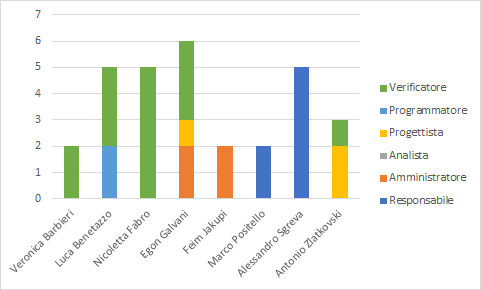
\includegraphics[width=0.7\textwidth]{./res/img/preventivi/inc22_po.png}
			\caption{Suddivisione oraria del 22$^{\circ}$ Incremento}
		\end{figure}
	
		\subsubsubsection{Prospetto economico}
		In base al prospetto orario, quello economico sarà il seguente: 
		\rowcolors{2}{lightRowColor}{darkRowColor}
		\begin{longtable}{
				>{\centering}p{0.25\textwidth}
				>{\centering}p{0.05\textwidth}
				>{\centering\arraybackslash}p{0.15\textwidth} }
			
			\coloredTableHead
			\textbf{\color{white}Ruolo} &
			\textbf{\color{white}Ore} &
			\textbf{\color{white}Costo in \euro{}}
			\tabularnewline
			\endhead
			
			% Contenuto della tabella
			% Ruolo & Ore & Costo \\
			Responsabile    & 7  & 210,00 \\
			Amministratore  & 4  & 80,00 \\
			Analista        & 0  & 0,00 \\
			Progettista     & 3  & 66,00 \\
			Programmatore   & 2  & 30,00 \\
			Verificatore    & 14  & 210,00 \\
			\textbf{Totale} & 30 & 596,00 \\
			
			\rowcolor{white}\caption {Prospetto dei costi per il 22$^{\circ}$ Incremento}	\\
			
		\end{longtable}
		
		% Grafico
		Rappresentazione grafica della distribuzione dei ruoli:
		\begin{figure}[H]
			\centering
			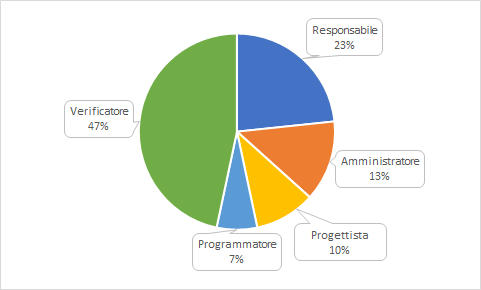
\includegraphics[width=0.7\textwidth]{./res/img/preventivi/inc22_pe.png}
			\caption{Prospetto economico del 22$^{\circ}$ Incremento}
		\end{figure}
	\pagebreak
	
	\begin{appendices}
\section{Riscontro dei rischi}
	\rowcolors{2}{lightRowColor}{darkRowColor}
	\begin{longtable}{
		>{\centering}p{0.1\textwidth}
		>{\centering}p{0.15\textwidth}
		>{\centering\arraybackslash}p{0.3\textwidth}
		>{\centering\arraybackslash}p{0.3\textwidth} }

		\caption {Riscontro dei rischi} \\

		\coloredTableHead
		\textbf{\color{white}ID} &
		\textbf{\color{white}Periodo} &
		\textbf{\color{white}Scenario} &
		\textbf{\color{white}Mitigazione}
		\tabularnewline
		\endhead

		% Contenuto della tabella
		% ID & Periodo & Scenario & Manutenzione migliorativa \\
		RT-1
		&
		Analisi
		&
		Molti componenti del gruppo \Gruppo{} non presentavano conoscenze pergresse di alcuni concetti e di molte delle tecnologie necessarie per lo sviluppo del progetto, come ad esempio l'ambiente\ped{\textit{G}} Serverless\ped{\textit{G}}, AWS\ped{\textit{G}}, Truffle\ped{\textit{G}} e il concetto di blockchain\ped{\textit{G}}
		&
		Il Proponente\ped{\textit{G}} e alcuni membri del gruppo che presentavano conoscenze pregresse in materia, si sono occupati di fornire materiale di studio in supporto agli altri membri del gruppo.\\

		RO-1
		&
		Analisi
		&
		A causa dell'inesperienza del gruppo nell'affrontare un progetto complesso, si sono presentati degli errori e delle cattive pratiche nello svolgimento del lavoro assegnato.
		&
		Il problema è stato mitigato dalla rotazione dei ruoli e dalle numerose riunioni che hanno permesso l'individuazione tempestiva e la correzione delle criticità sopracitate.\\
\hline
		RO-1
		&
		Progettazione Architetturale
		&
		A causa dell'inesperienza del gruppo non è stato semplice ed immediato riuscire a capire a fondo le indicazioni ricevute nell'esito della \textit{Revisione dei Requisiti} riguardo l'errata adesione al modello incrementale.
		&
		La collaborazione tra i componenti del gruppo, tramite esposizione dei propri dubbi e delle proprie perplessità, e uno studio più approfondito del modello incrementale hanno permesso di colmare le lacune dovute all'inesperienza e di risolvere questo problema.\\

		RO-1
		&
		Progettazione Architetturale
		&
		Sono state rilevate alcune difficoltà nell'organizzare il lavoro e nella rotazione dei ruoli.
		La difficoltà maggiore per i componenti del gruppo è stata riscontrata nel passaggio da un ruolo ad un altro, dovendo quindi ambientarsi nel nuovo ruolo ed organizzarsi per continuare il lavoro svolto da un altro componente del gruppo.
		&
		Per limitare il più possibile eventuali ritardi dovuti alla rotazione dei ruoli ciascun componente del gruppo ha tempestivamente comunicato agli altri, durante le frequenti riunioni interne, eventuali problematiche riscontrate per fare in modo di risolverle con l'aiuto di coloro i quali hanno già svolto quello stesso ruolo in precedenza.
		Questo approccio si è rivelato molto efficace, perché ha limitato la possibilità che errori simili o identici si siano verificati a seguito delle varie rotazioni. \\

		RO-3
		&
		Progettazione Architetturale
		&
		A causa di esami universitari o di altri impegni personali, alcuni componenti non sono riusciti a portare a termine alcuni compiti assegnati entro una certa scadenza, concordata all'interno del gruppo.
		&
		Per ridurre al minimo eventuali ritardi dovuti a questa problematica ciascun componente ha notificato per tempo al resto del gruppo il proprio impegno ed il gruppo si è organizzato ridistribuendo il lavoro ad altri componenti per riuscire a portare a termine quel compito entro la scadenza prefissata.  \\

		RI-1
		&
		Progettazione Architetturale
		&
		Durante alcune riunioni interne svolte in questo periodo nelle quali sono state prese delle decisioni talvolta importanti, alcuni componenti non hanno potuto partecipare all'incontro o sono dovuti uscire prima della fine.
		&
		Durante ciascuna riunione interna è stata decisa e concordata la data e l'ora della riunione successiva, in modo da notificare immediatamente eventuali momenti di irreperibilità e di riuscire ad essere tutti presenti all'incontro successivo.
		A seguito dell'impossibilità per un componente di partecipare ad un incontro, quest'ultimo ha sempre comunicato preventivamente l'avanzamento del proprio lavoro ed eventuali quesiti da porre, permettendo quindi al Responsabile si riportare tali infomazioni durante l'incontro.
		Per ciascun incontro è stato sempre nominato un Segretario col compito di redigere un verbale con tutto ciò che è stato detto e tutte le decisioni prese. Il componente assente ha perciò potuto informarsi sulle discussioni avvenute durante l'incontro, leggendo il relativo verbale. \\
\hline
		RO-3
		&
		Progettazione di dettaglio e codifica
		&
		A causa di esami universitari o di altri impegni personali, alcuni componenti non sono riusciti a portare a termine alcuni compiti assegnati entro una certa scadenza, oppure non hanno potuto presenziare agli incontri di gruppo.
		&
		Per ridurre al minimo eventuali ritardi dovuti a queste problematiche, ciascun componente ha notificato per tempo il resto del gruppo per potersi organizzare ridistribuendo il lavoro e portando a termine quel compito entro la scadenza prefissata.  \\

		RT-1
		&
		Progettazione di dettaglio e codifica
		&
		Si sono presentate alcune lacune nella conoscenza approfondita delle tecnologie scelte, in particolare nell'ambiente di testing del codice del prodotto.
		&
		I membri del gruppo, data l'esperienza accumulata nel trascorrere del progetto, si sono documentati sugli argomenti nei quali presentassero lacune, presentando poi i risultati ottenuti al resto del gruppo.\\

		RT-4
		&
		Progettazione di dettaglio e codifica
		&
		Si sono presentate alcune lacune nella conoscenza dei design pattern e degli stili architetturali, necessari per ottenere una progettazione efficace del prodotto. I Progettisti si sono documentati sugli argomenti, anche in seguito alle indicazioni ricevute in riunione con il \RC{}. Tuttavia alcuni design pattern non sono stati implementati correttamente, nello specifico \textit{Facade} e \textit{Command}. Questi errori quindi, mancati al rilevamento, sono stati riportati anche in sede di Product Baseline, dove sono stati evidenziati dal professore.
		&
		I Progettisti si sono immediatamente impegnati a rivalutare e correggere l'implementazione dei design pattern e di conseguenza la progettazione del modulo in questione. Collaborando strettamente verranno ridotti al minimo i ritardi causati dalla problematica.\\
	\end{longtable}
\end{appendices}

	\pagebreak
	
	\begin{appendices}
\section{Organigramma}
	\subsection{Redazione}
		\rowcolors{2}{lightRowColor}{darkRowColor}
		\begin{longtable}{
			>{\centering}p{0.25\textwidth}
			>{\centering}p{0.15\textwidth}
			>{\centering\arraybackslash}p{0.25\textwidth} }

			\coloredTableHead
			\textbf{\color{white}Nome} &
			\textbf{\color{white}Data} &
			\textbf{\color{white}Firma}
			\tabularnewline
			\endhead

			% Contenuto della tabella
			% Nome & Data & Firma\\
			\MP & - & 
\includegraphics[width=0.2\textwidth]{./res/img/FirmeComponenti/firma_MP.jpg} \\
			\VB & - & 
\includegraphics[width=0.2\textwidth]{./res/img/FirmeComponenti/firma_VB.jpg} \\

			\rowcolor{white}\caption {Redazione}	\\

		\end{longtable}

	\subsection{Approvazione}
		\rowcolors{2}{lightRowColor}{darkRowColor}
		\begin{longtable}{
			>{\centering}p{0.25\textwidth}
			>{\centering}p{0.15\textwidth}
			>{\centering\arraybackslash}p{0.25\textwidth} }

			\coloredTableHead
			\textbf{\color{white}Nome} &
			\textbf{\color{white}Data} &
			\textbf{\color{white}Firma}
			\tabularnewline
			\endhead

			% Contenuto della tabella
			% Nome & Data & Firma\\
			- & - & - \\
			\TV & - & - \\

			\rowcolor{white}\caption {Approvazione} \\

		\end{longtable}
\newpage
	\subsection{Accettazione dei componenti}
		\rowcolors{2}{lightRowColor}{darkRowColor}
		\begin{longtable}{
			>{\centering}p{0.25\textwidth}
			>{\centering}p{0.15\textwidth}
			>{\centering\arraybackslash}p{0.25\textwidth} }

			\coloredTableHead
			\textbf{\color{white}Nome} &
			\textbf{\color{white}Data} &
			\textbf{\color{white}Firma}
			\tabularnewline
			\endhead

			% Contenuto della tabella
			% Nome & Data & Firma\\
			\VB & 2020-03-12 & 
\includegraphics[width=0.25\textwidth]{./res/img/FirmeComponenti/firma_VB.jpg} \\
			\NF & 2020-03-12 & 
\includegraphics[width=0.2\textwidth]{./res/img/FirmeComponenti/firma_NF.jpg} \\
			\EG & 2020-03-12 & 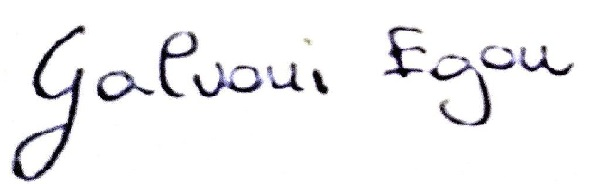
\includegraphics[width=0.2\textwidth]{./res/img/FirmeComponenti/firma_EG.jpg} \\
			\FJ & 2020-03-12 & 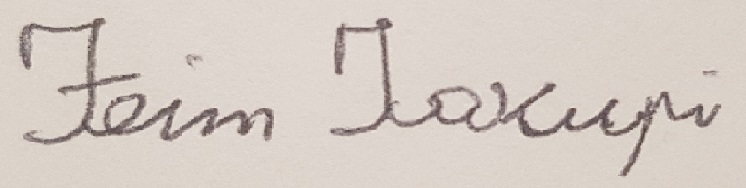
\includegraphics[width=0.2\textwidth]{./res/img/FirmeComponenti/firma_FJ.jpg} \\
			\MP & 2020-03-12 & 
\includegraphics[width=0.2\textwidth]{./res/img/FirmeComponenti/firma_MP.jpg} \\
			\LB & 2020-03-12 & 
\includegraphics[width=0.2\textwidth]{./res/img/FirmeComponenti/firma_LB.jpg} \\
			\AS & 2020-03-12 & 
\includegraphics[width=0.2\textwidth]{./res/img/FirmeComponenti/firma_AS.jpg} \\
			\AZ & 2020-03-12 & 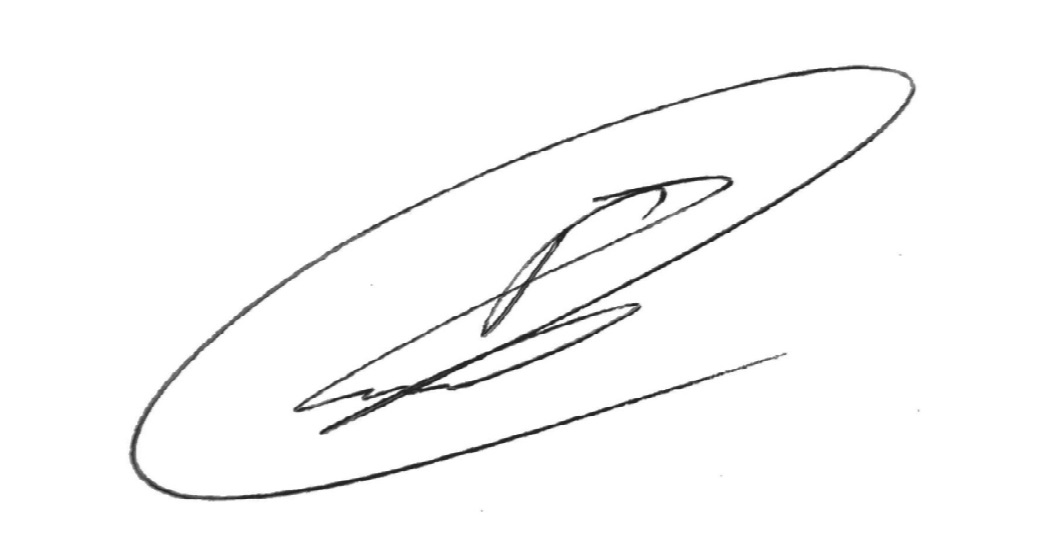
\includegraphics[width=0.2\textwidth]{./res/img/FirmeComponenti/firma_AZ.jpg} \\

			\rowcolor{white}\caption {Accettazione dei componenti} \\

		\end{longtable}

	\subsection{Componenti}
		\rowcolors{2}{lightRowColor}{darkRowColor}
		\begin{longtable}{
			>{\centering}p{0.25\textwidth}
			>{\centering}p{0.15\textwidth}
			>{\centering\arraybackslash}p{0.4\textwidth} }

			\coloredTableHead
			\textbf{\color{white}Nome} &
			\textbf{\color{white}Matricola} &
			\textbf{\color{white}Indirizzo email}
			\tabularnewline
			\endhead

			% Contenuto della tabella
			% Nome & Matricola & Indirizzo email\\
			\VB & 1143463 & veronica.barbieri.1@studenti.unipd.it \\
			\LB & 1122109 & luca.benetazzo@studenti.unipd.it \\
			\NF & 1143541 & nicoletta.fabro@studenti.unipd.it \\
			\EG & 1187021 & egon.galvani@studenti.unipd.it \\
			\FJ & 1163064 & feim.jakupi@studenti.unipd.it \\
			\MP & 1167693 & marco.positello@studenti.unipd.it \\
			\AS & 1144363 & alessandro.sgreva@studenti.unipd.it \\
			\AZ & 1171766 & antonio.zlatkovski@studenti.unipd.it \\

			\rowcolor{white}\caption {Componenti} \\

		\end{longtable}
\end{appendices}

	\pagebreak
	
\end{document}